% arara: xelatex
% arara: xelatex
% arara: xelatex


% options:
% thesis=B bachelor's thesis
% thesis=M master's thesis
% czech thesis in Czech language
% english thesis in English language
% hidelinks remove colour boxes around hyperlinks

\documentclass[thesis=M,english]{FITthesis}[2019/03/06]

%\usepackage[utf8]{inputenc} % LaTeX source encoded as UTF-8
% \usepackage[latin2]{inputenc} % LaTeX source encoded as ISO-8859-2
% \usepackage[cp1250]{inputenc} % LaTeX source encoded as Windows-1250

% \usepackage{subfig} %subfigures
% \usepackage{amsmath} %advanced maths
% \usepackage{amssymb} %additional math symbols

\usepackage{dirtree} %directory tree visualisation
\usepackage{csquotes}
\usepackage[table,xcdraw]{xcolor}
\usepackage{spverbatim}
\usepackage{amsfonts}
\usepackage{blindtext}
\usepackage{pdfpages}
\usepackage{amsmath}
\usepackage[section]{placeins}
\usepackage{underscore}
\usepackage{minted}
\usepackage{rotating}
\usepackage[T1]{fontenc}
\usepackage{eurosym}
\usepackage[ruled,vlined]{algorithm2e}
\usepackage[noend]{algpseudocode}
% % list of acronyms
% \usepackage[acronym,nonumberlist,toc,numberedsection=autolabel]{glossaries}
% \iflanguage{czech}{\renewcommand*{\acronymname}{Seznam pou{\v z}it{\' y}ch zkratek}}{}
% \makeglossaries

% % % % % % % % % % % % % % % % % % % % % % % % % % % % % % 
% EDIT THIS
% % % % % % % % % % % % % % % % % % % % % % % % % % % % % % 

\department{Department of Software Engineering}
\title{Parking lot detection system}
\authorGN{Ji{\v r}í} %author's given name/names
\authorFN{Groh} %author's surname
\author{Ji{\v r}í Groh} %author's name without academic degrees
\authorWithDegrees{Bc. Ji{\v r}í Groh} %author's name with academic degrees
\supervisor{Ing. Marek Su{\v s}ick{\' y}}
\abstractEN{Goal of this work is to design and implement autonomous system that extracts parking spots on a parking lot from a video stream and continuously monitor and gather the occupancy status of the parking lot over time.}
\abstractCS{C\'{\i}lem t\'{e}to pr\'{a}ce je navrhnout a implementovat autonomn\'{\i} syst\'{e}m, kter\'{y} extrahuje parkovac\'{\i} m\'{\i}sta na parkovi\v{s}ti ze streamovan\'{e}ho kamerov\'{e}ho z\'{a}znamu. Syst\'{e}m tak\'{e} vyhodnocuje a zaznamen\'{a}v\'{a} obsazenost parkovi\v{s}t\v{e} v \v{c}ase.
}
\placeForDeclarationOfAuthenticity{Prague}
\keywordsCS{Replace with comma-separated list of keywords in Czech.}
\keywordsEN{Replace with comma-separated list of keywords in English.}
\declarationOfAuthenticityOption{1} %select as appropriate, according to the desired license (integer 1-6)
% \website{http://site.example/thesis} %optional thesis URL


\begin{document}

% \newacronym{CVUT}{{\v C}VUT}{{\v C}esk{\' e} vysok{\' e} u{\v c}en{\' i} technick{\' e} v Praze}
% \newacronym{FIT}{FIT}{Fakulta informa{\v c}n{\' i}ch technologi{\' i}}

\setsecnumdepth{part}
\chapter{Introduction}
The goal of this work is to design a solution that will be able to detect parking lot occupancy status from a camera video feed. \\

Solution is not reliant on existing roadway markings and uses object detection to find stationary cars in the parking lot. The location of these stationary cars is being used as the reference for further classification of the status of the parking space. \\

Whole architecture of the system is able to support multiple cameras running in mutually disjoint fields of view.\\

Output is be displayed in web based application in the form of statistics about parking lot and its parking spots as well as it's configuration.\\



All the work is open source under the auspices of OpenDataLab.




\setsecnumdepth{all}
\chapter{Analysis}
\section{Law compliance}
Camera footage of a parking lot can and eventually will contain images of people that can be directly or indirectly identified, thus becoming a personal data. Each country has different policy and laws concerning personal data, such as protection, usage and storage.\\

For the purpose of this work it is assumed that the camera responsible for providing footage is placed legally and lawfully and the integrator has permit to use the footage for processing.\\

The implementation of this system will not persist any camera footage.


\section{Existing solutions}
Measuring the occupancy of parking lots is widely used today, good example would be a shopping mall garage. Plenty of them have a screen at the entrance indicating the number of vacant parking spots.\\

Most of these occupancy detection systems rely on external hardware that of course isn't free. Arguably, the price of these systems is insignificant in comparison with the cost of the whole building. However, the building plans have to account for accommodation of such system. Meaning that adding this detection later on could require significant intervention. The external hardware is usually infrared or ultrasonic sensor that detects presence of a car.\\


\subsection{DeepParking}
DeepParking\footnote{\url{https://github.com/DeepParking/DeepParking}} is an open source system for detection vacant parking spots in parking garages. The solution relies on low-cost cameras mounted to the garage with manually predefined locations of parking spaces. The solution also offers navigation to an empty parking space via notifications.\\

The authors recommend up to five parking spots managed by single static camera or up to ten parking spots for camera with ability to rotate. The system utilizes You Only Look Once (YOLO) object detector.\\


The authors estimate the cost for garage of 100 spaces to be around \$150.
\subsection{ParkingDetection}

ParkingDetection is a commercial product developed by Czech company RCE Systems s.r.o. The system itself not only supports parking lot occupancy from the camera feed but also allows to collect parking fees and see time-based statistics about the parking lot. This software can take advantage of an existing camera surveillance. \\

The company is using AI based systems and claims to detect up to 400 unmarked parking spaces from a single camera. The video feed is processed every second achieving almost real-time results. Advertised delay is in order of minutes.\\

However, this product is not open source, so the actual implementation specifics are unknown. The pricing is about 77 EUR per parking spot.




\section{Detection of parking spaces}
Parking spot detection is one of the challenges in this work. The task is to process camera footage and extract location of the parking spots in the image.
\\ 

There is a wide variety of parking lot designs, where features of one lot aren't always the features of another lot. That makes this problem very hard to solve let alone from single camera image.
\\



An example of such feature could be markings on the road, white or yellow lines drawn onto the surface. They are the straight forward delimitation of a parking space, but are not present generally. It is very common to see parallel parking on the street without any sort of road markings.
\\


A very good indicator of parking lot is the car itself. Modern state-of-the-art image detectors are able to locate a car in an image with very high accuracy. Locating a stationary car using this technique and assuming that the car is parked correctly between the lines would be a very good estimation of the actual parking spot location. The obvious disadvantage is that there needs to be a car present first in order to detect a parking spot.
\\


There are also another caveats to this approach, such as people parking at places where they lawfully should not. These problems will need to be addressed in later processing of acquired data.



\subsection{State-of-the-art object detectors}
Object detection is a computer vision discipline specialized in detecting multiple instances of particular objects\footnote{Also known as classes.} as well as their location in the image. The location of the object is usually determined as axis aligned bounding box (AABB) or a mask that approximates the shape of the detected object.\\

Modern object detectors utilize deep learning. More specifically tens or hundreds of hidden layers composed of convolutional and dense layers along with techniques such as pooling, dropout, activation functions, etc. Characteristics of these layers and concepts will be briefly summarized. The training algorithms and back propagation will not be discussed.

\subsubsection{Dense layer}
Dense layer containing $n \in \mathbb{N}$ units\footnote{Sometimes referred to as neurons.} where each unit in a layer is connected to every unit from previous layer. Illustration of that can be seen in Figure \ref{label:dense_layers}. Each connection between units is weighted and each unit has its own bias. Output j-th unit in l-th layer is defined by following  formula.
$$ a_{j}^l = f(\sum_k w^l_{jk} * a^{l-1}_{k} + b^l_j) $$
Where \(w^l_{jk}\) is weight between k-th unit in l-th layer and j-th unit in l-th layer, \(b^l_j\) is bias of j-th unit in l-th layer and \(f\) is an activation function \cite{nielsenneural}.

\begin{figure}[!ht]
	\centering
	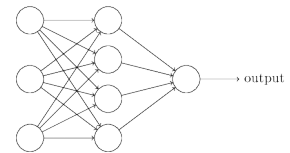
\includegraphics[width=0.4\textwidth]{imgs/dense-example.png}
	\caption{Example of three connected dense layers \cite{nielsenneural}.}
	\label{label:dense_layers}
\end{figure}

\subsubsection{Convolutional layer}
Convolutional layers are better adapted to retain spatial information from the input, that is very important when it comes to processing images and generalization of the intended problem. M. Nielsen says in his book \enquote{But
upon reflection, it’s strange to use networks with fully-connected layers to classify images.
The reason is that such a network architecture does not take into account the spatial structure
of the images. For instance, it treats input pixels which are far apart and close together
on exactly the same footing.} \cite{nielsenneural} \\

In this layer its better to think about the input as a
multidimensional matrix. It can very well be an image interpreted in (width, height, RGB values = depth) format. The convolutional layer uses kernel matrix\footnote{Also known as feature extractor.} of size S x S that is being slid over the input in a given stride length to produce output called feature map. An example of this can be seen in Figure \ref{label:kernel_sliding}. \\



That way each unit in following layer has bias and S x S weight matrix allocated to the corresponding part of the input. The bias and the weight matrix are shared across all units in the feature map, that means they are able to detect the same \enquote{feature} in the image.\\

When the convolution layer is followed by dense layer, the output is usually flattened into single column matrix - a vector. \\

The value of j,k-th unit in following layer l is expressed as following.

$$ a^{l}_{j,k} = f(\sum^S_{m=0} \sum^S_{n=0} w^l_{m,n} a^{l-1}_{j+m, k+n} + b) $$

Where \(f\) is again an activation function, \(w^l_{m,n}\) are the shared weights for units in particular feature map and \(b\) is the shared bias.



\subsubsection{Pooling layers}
Pooling layer also uses sliding kernel S x S with specified stride length to perform operations on the corresponding part of the input. This simplifies the information from the previous layer and also provides translational invariance (to some degree), meaning that the result is not affected by slight image inconsistencies.\\


\begin{description}
    \item [\textbf{Most common used operations in pooling layer are following:}]
    \item [Max Pooling] Extracts the maximum value from window.
    \item [Min Pooling] Extracts the minimum value from window.
    \item [Avg Pooling] Extracts the average value from the window.
    \end{description}
    
\begin{figure}[ht]
	\centering
	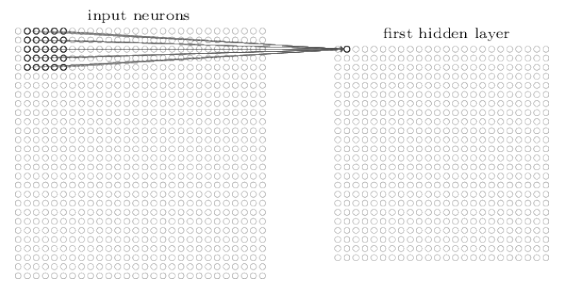
\includegraphics[width=0.9\textwidth, height=0.4\textwidth]{imgs/conv-example.png}
	\caption{Example of sliding kernel (5x5) producing extracing a feature map (24x24) from input (28x28) \cite{nielsenneural}.}
	\label{label:kernel_sliding}
\end{figure}



\subsection{Activation Functions}
As described above, the activation functions are applied to the output of a neuron (unit). The main goal of using such function is to bind the output value to some domain and to introduce non-linearity to the network in order to increase its potential to approximate functions, therefore increasing the ability to learn.

Few of the most used activation functions will be discussed.


\subsubsection{Sigmoid}
Sigmoid is one of the widely used activation function that binds the output between zero and one. Using this function can introduce the problem of vanishing gradient during training of the network due to its quick convergence towards one and zero, making the changes during learning insignificant.
$$
\sigma(x) = \frac{1}{1-e^{-x}}
$$
\subsubsection{Tanh}
Hyperbolic tangent $tanh(x)$ is very similar to the sigmoid function and it binds the output between -1 and 1. This function can also introduce the problem of vanishing gradient for the same reason as the sigmoid function. 


\subsubsection{ReLU}

ReLU stands for rectified linear unit and is widely used in deep learning field. This function reduces the problem of vanishing gradient.
$$
ReLU(x) = max(0,x)
$$
As can be seen from the equation, the negative input always results in 0 on the output which can cause a dead neuron problem. Solution to this problem is a parametric ReLU that introduces the parameter $a$. For example, in the leaky ReLU the parameter is set $a = 0.01$ to create a slight slope for $x < 0$.


 \begin{equation}
    Parametric ReLU(x) =
    \begin{cases}
      x, & \text{if}\ x > 0 \\
      ax, & \text{otherwise}
    \end{cases}
  \end{equation}
\subsubsection{Softmax}
Softmax is an activation function that is usually used in the last (output) layer to normalize the output vector into a vector of probabilities, where the sum is equal to 1. This function is often used in classification problems.
$$ softmax(x)_i = \frac{exp(x_i)}{\sum_{j}^{ }exp(x_j)} $$


\begin{table}[ht!]
\centering
\caption{Example of softmax function.}
\begin{tabular}{|l|l|l|}
\hline
\multicolumn{1}{|c|}{\textbf{$x$}} & \multicolumn{1}{c|}{\textbf{$e^x$}} & \multicolumn{1}{c|}{\textbf{$softmax(x)$}} \\ \hline
{\color[HTML]{000000} 1}             & {\color[HTML]{000000} 2.718281828}                     & {\color[HTML]{000000} 0.000004086453048}     \\ \hline
{\color[HTML]{000000} 13}            & {\color[HTML]{000000} 442413.392}                      & {\color[HTML]{000000} 0.6650898135}          \\ \hline
{\color[HTML]{000000} 11}            & {\color[HTML]{000000} 59874.14172}                     & {\color[HTML]{000000} 0.09001011829}         \\ \hline
{\color[HTML]{000000} 12}            & {\color[HTML]{000000} 162754.7914}                     & {\color[HTML]{000000} 0.2446728689}          \\ \hline
{\color[HTML]{000000} 5}             & {\color[HTML]{000000} 148.4131591}                     & {\color[HTML]{000000} 0.0002231127766}       \\ \hline
\end{tabular}
\end{table}
\subsection{Examined object detectors}
This chapter is focused on the most prominent and powerful object detectors available in the time of writing this work. An assumption was made, that fast and precise object detector is crucial for this work in order to achieve real-time evaluation. 
\subsubsection{Mask R-CNN}
Mask R-CNN comes from the family of R-CNNs (Region based Convolutional Neural Networks).\\

R-CNN relies on underlying algorithm to propose regions of interest. Each region is fed to CNN (Convolutional Neural Network) to extract features. Finally those features are fed into SVM (Support Vector Machine) in order to be classified. This approach turns out to be quite accurate, but the whole pipeline is slow even on a powerful GPU card (47 seconds of inference time per image) \cite{rcnn} \cite{fast-rcnn}.\\

Next iteration of R-CNN is Fast R-CNN. Fast R-CNN uses CNN to produce feature maps from the whole image at once. Then the regions of interest are pooled accordingly to a corresponding proposed region from the feature maps. Fast R-CNN achieves slight improvement in mean average precision (mAP)\footnote{mAP is the mean of average precisions in multiple class classification} and significant boost in speed (around 2 seconds of inference time per image) \cite{fast-rcnn}.\\

Next improvement is called Faster R-CNN. In previous iterations the bottleneck was the region proposal algorithm. That was solved in Faster R-CNN by introducing FCNN (Fully Convolutional Neural Network) more specifically RPN (Region Proposal Network). A separate network that is trained to predict region proposals. Faster R-CNN is about 250 times faster than the original R-CNN achieving almost real-time performance at 47 images per second \cite{faster-rcnn}.






\subsubsection{YOLO}
YOLO (You Only Look Once) is a object detector that approaches the problem a bit differently than the R-CNN family networks mentioned above. It treats the object detection as a single regression problem, therefore no complex pipeline is required. The input image is divided into $S \times S$ grid and each cell is responsible for predicting $B$ bounding boxes, confidence of these boxes and class probability of the object. First iteration of YOLO achieved very high performance (45 images per second) and 63.4 mAP. However, it poses a limit on how much bounding boxes can be predicted by single grid cell \cite{yolov1}.  \\

Another two papers with improvements of YOLO were published, namely addressing the shortcomings of the original implementation, while increasing the mAP and performance of the network \cite{yolov2} \cite{redmon2018yolov3}.

\subsubsection{Comparison}
Implementations of both object detectors mentioned above were used for comparison to determine their ability to detect cars on total of five representational samples. Four of these samples were obtained from videos recorded by the author and one was taken from a video of parking lot from the internet (processed and compressed). The videos cover differents heights of the camera to determine the ability to detect cars from both side and top view with different sizes and granularity. \\

The performance was measured strictly for the ability to detect vehicles present in the image. Both detectors do recognize cars and trucks separately, but in this case they are treated as the same object. There are four possible outcomes possible in this measure.

\begin{enumerate}
    \item True positive (TP) - the bounding box contains a vehicle and it is classified as a vehicle.
    \item False negative (FN) - the bounding box contains a vehicle but it is not classified as a vehicle.
    \item False positive (FP) - the bounding box does not contain vehicle and it is classified as a vehicle.
    \item Not detected (ND) - a vehicle was not detected at all.
\end{enumerate}

The overview of results on all five videos can be seen in Figure \ref{label:comparison_graph}. The detection preview for each chart may be seen in Figures \ref{label:comparison_fhd}, \ref{label:comparison_hd}, \ref{label:comparison_raspi},  \ref{label:comparison_ytvid}, \ref{label:comparison_np} respectively.\\

The Mask R-CNN performs better than YOLO in finding vehicles in first two footages with higher resolution, but also makes more mistakes in classifying the objects, notably mistaking the building for a truck. In the footage from Raspberry Pi camera where the resolution is lower and quality is poorer the YOLOv3 detector performed much better in classification of the vehicles, while also predicting the whole parking lot to be a keyboard.\\

In videos where the camera was placed closer to the ground both models performed very similarly. Nevertheless, Mask R-CNN was able to detect finer objects in the image.

\begin{figure}[!htb]
	\centering
	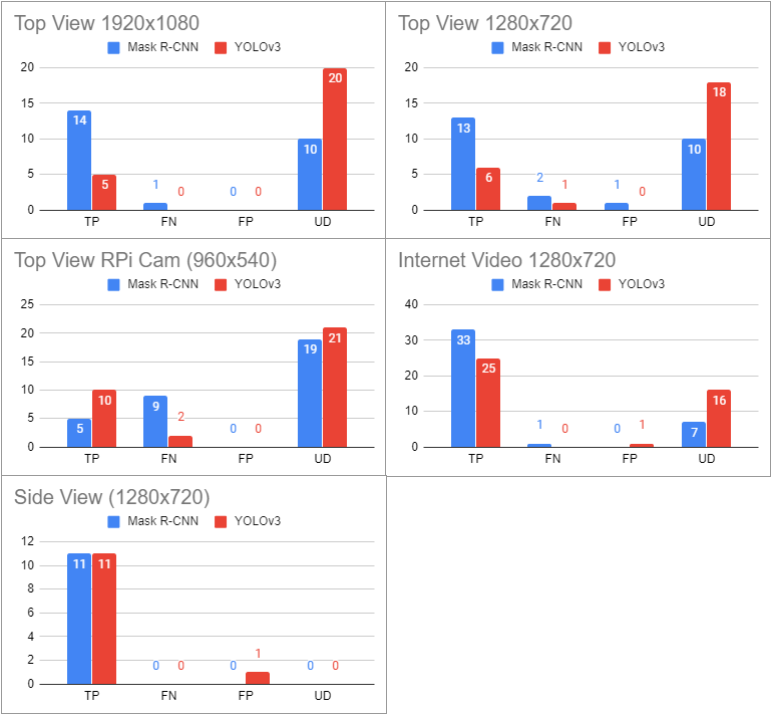
\includegraphics[width=0.90\textwidth]{imgs/graphs.png}
	\caption{Detection results of Mask R-CNN and YOLOv3 on all five videos.}
	\label{label:comparison_graph}
\end{figure}
\begin{figure}[!htb]
	\centering
	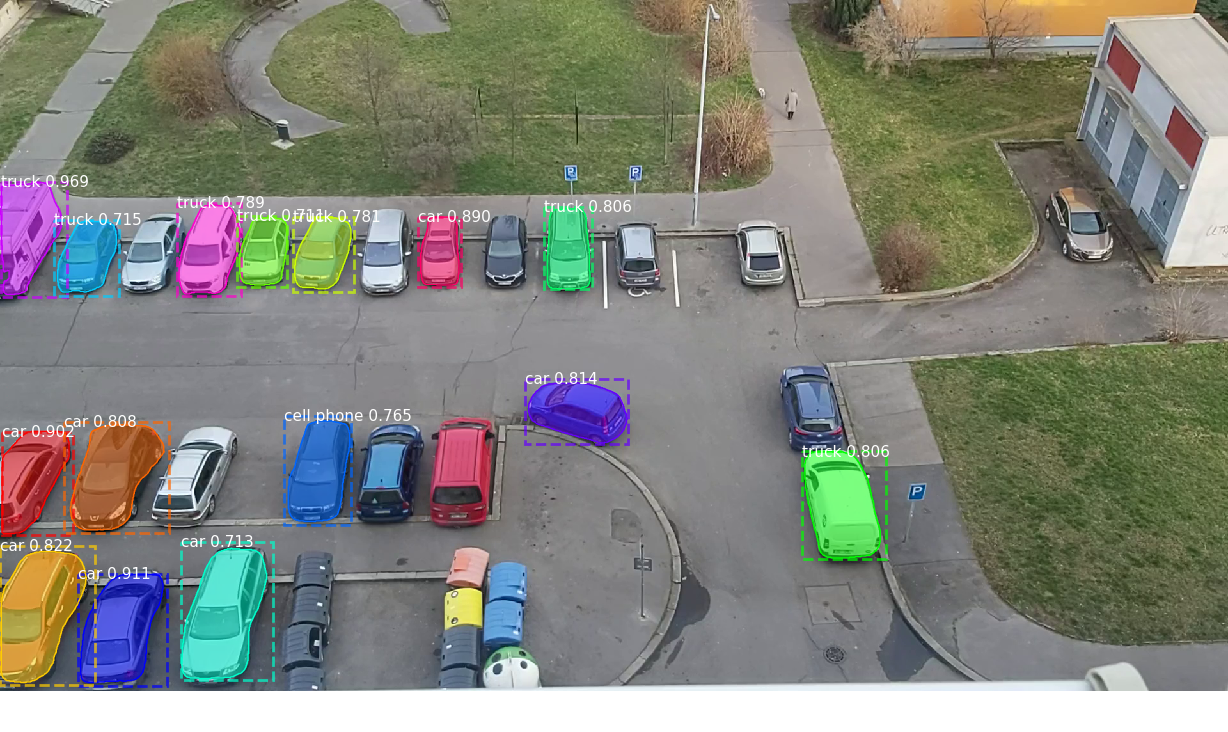
\includegraphics[width=0.90\textwidth]{imgs/mask-fhd.png}
	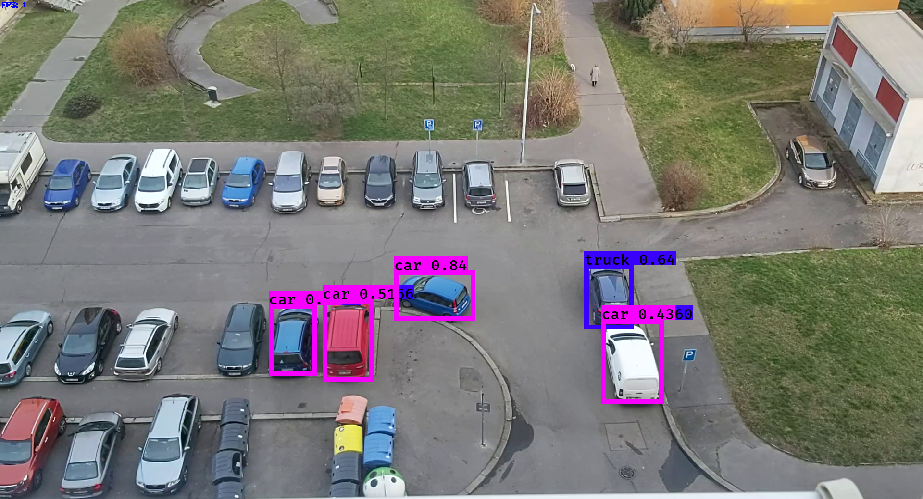
\includegraphics[width=0.90\textwidth]{imgs/yolo-fhd.png}
	\caption{Detection results of Mask R-CNN (top) and YOLOv3 (bottom) on 1920x1080 top view footage. Source: author.}
	\label{label:comparison_fhd}
\end{figure}

\begin{figure}[!htb]
	\centering
	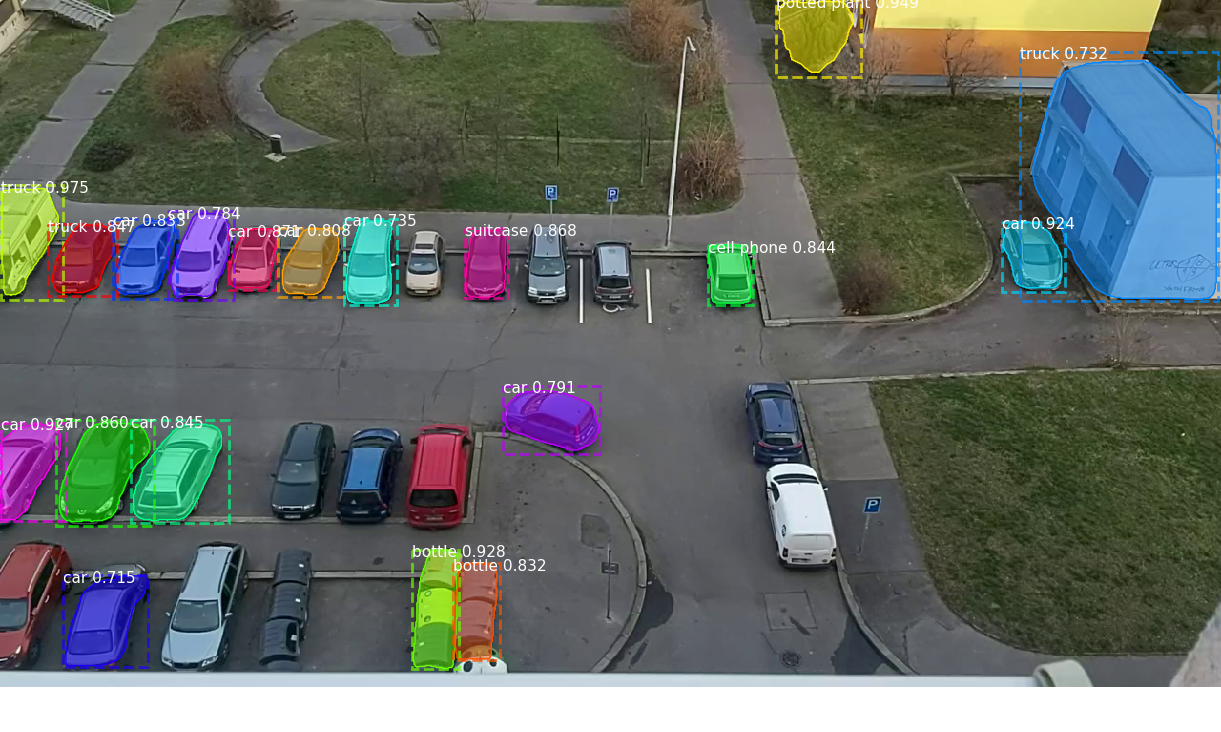
\includegraphics[width=0.90\textwidth]{imgs/mask-hd.png}
	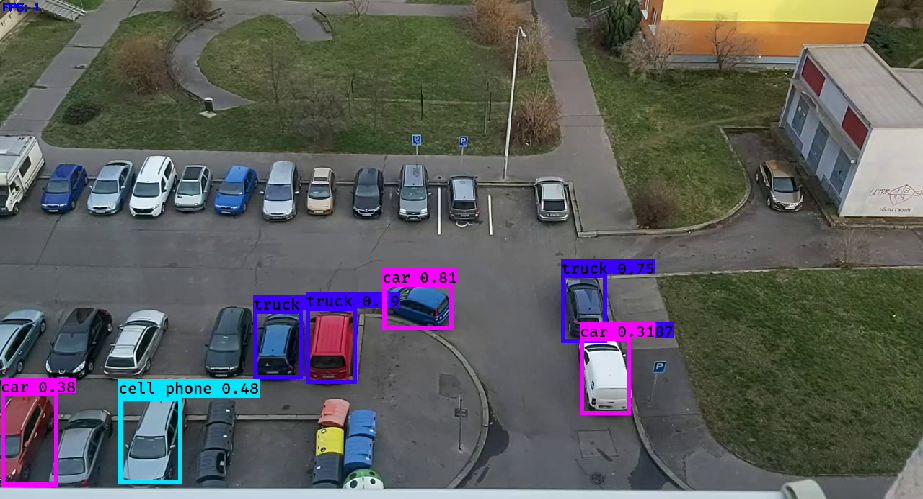
\includegraphics[width=0.90\textwidth]{imgs/yolo-hd.png}
	\caption{Detection results of Mask R-CNN (top) and YOLOv3 (bottom) on 1920x1080 top view footage. Source: author.}
	\label{label:comparison_hd}
\end{figure}


\begin{figure}[!htb]
	\centering
	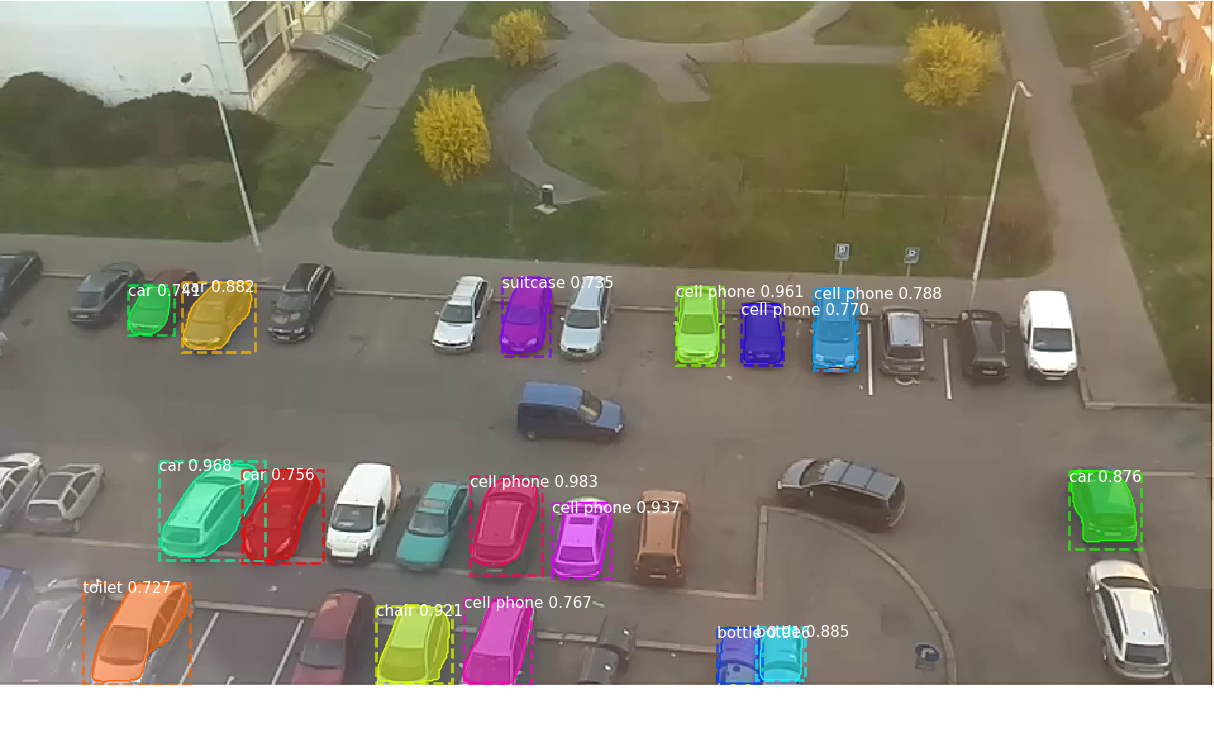
\includegraphics[width=0.90\textwidth]{imgs/mask-raspi.png}
	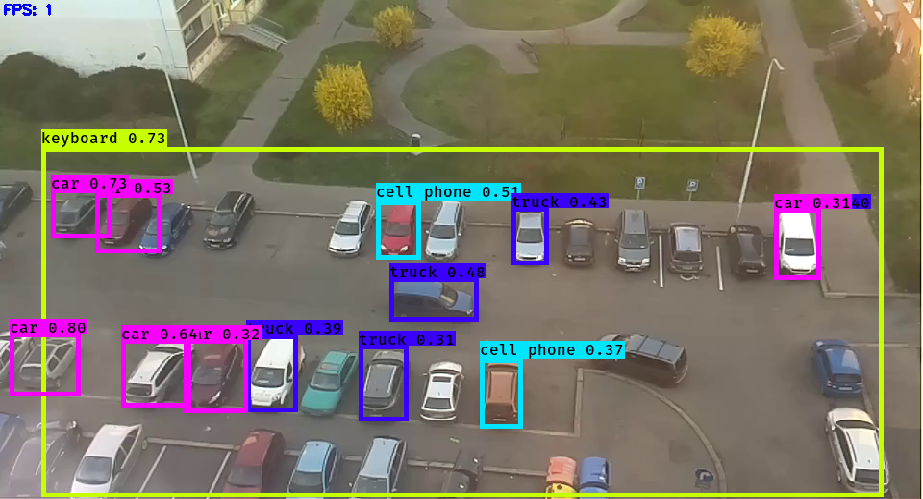
\includegraphics[width=0.90\textwidth]{imgs/yolo-raspi.png}
	\caption{Detection results of Mask R-CNN (top) and YOLOv3 (bottom) on 960x540 of top view footage from the Raspberry Pi Camera. Source: author.}
	\label{label:comparison_raspi}
\end{figure}

\begin{figure}[!htb]
	\centering
	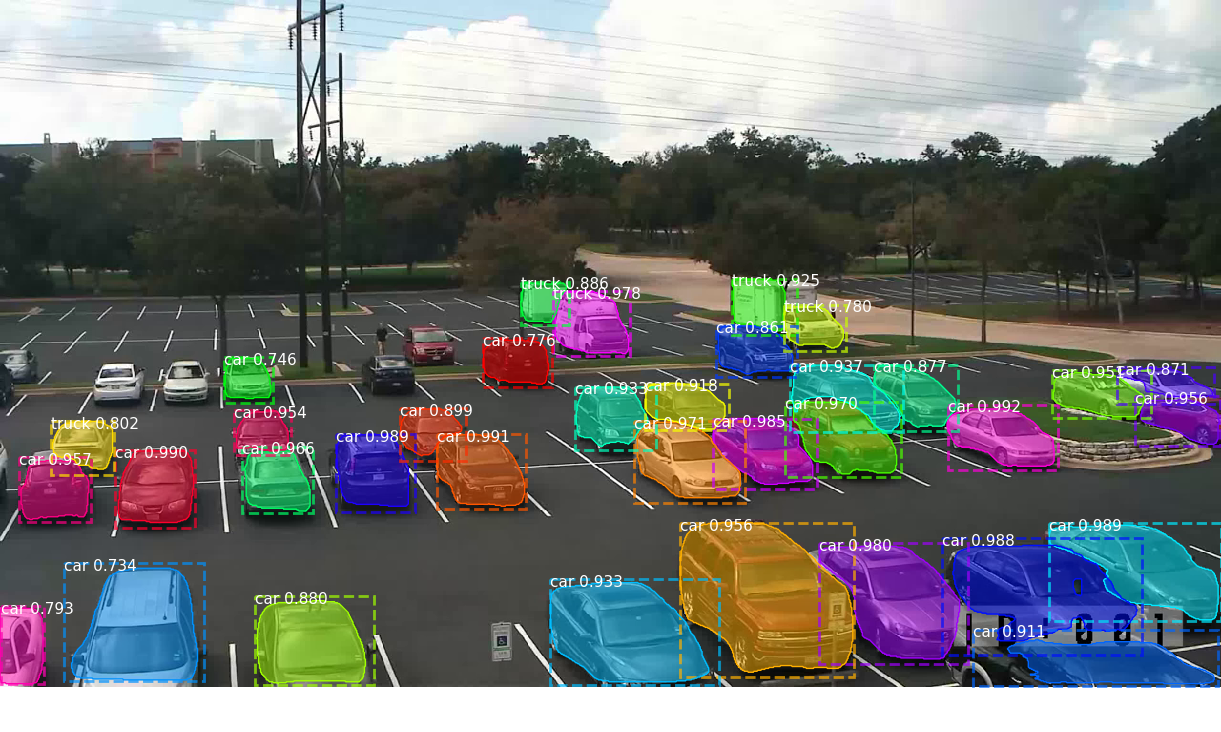
\includegraphics[width=0.90\textwidth]{imgs/mask-ytvid.png}
	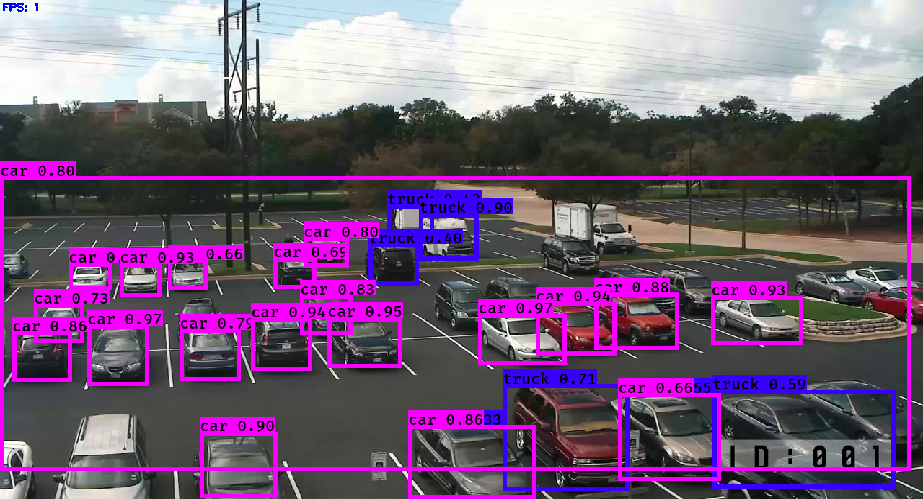
\includegraphics[width=0.90\textwidth]{imgs/yolo-ytvid.png}
	\caption{Detection results of Mask R-CNN (top) and YOLOv3 (bottom) on 1280x720 side view with wider angle. Source: author.}
	\label{label:comparison_ytvid}
\end{figure}

\begin{figure}[!htb]
	\centering
	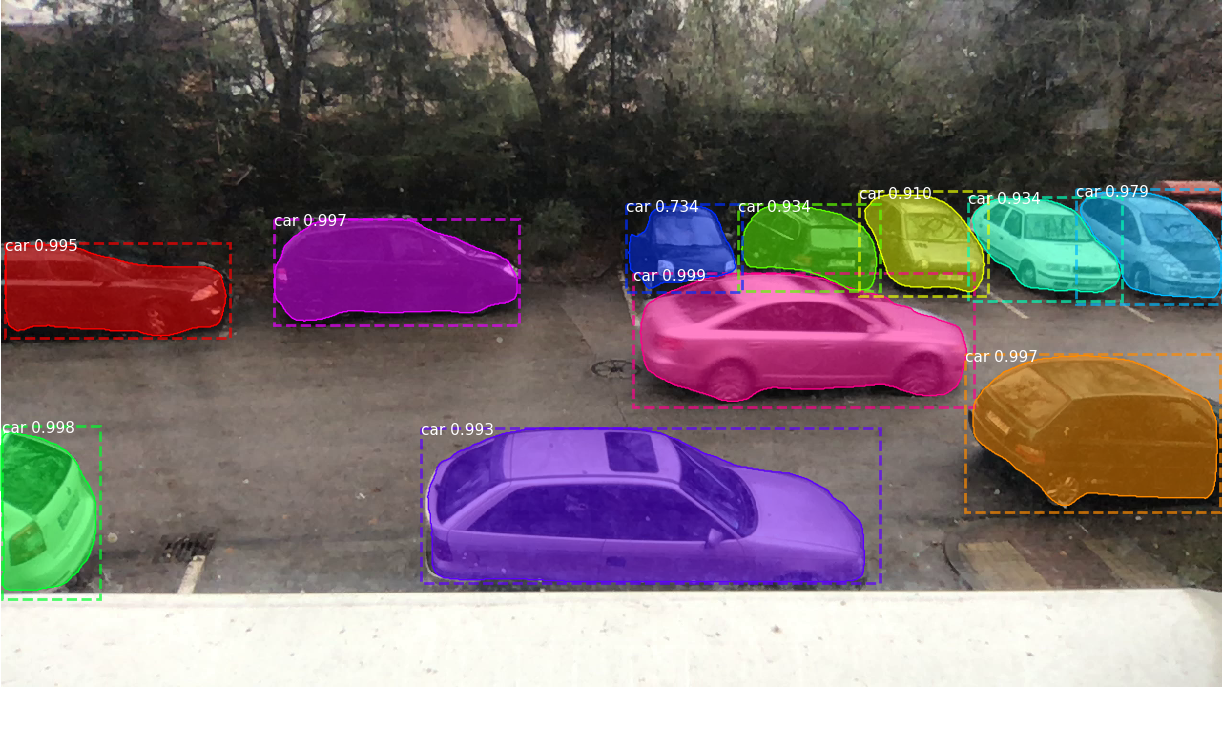
\includegraphics[width=0.90\textwidth]{imgs/mask-np.png}
	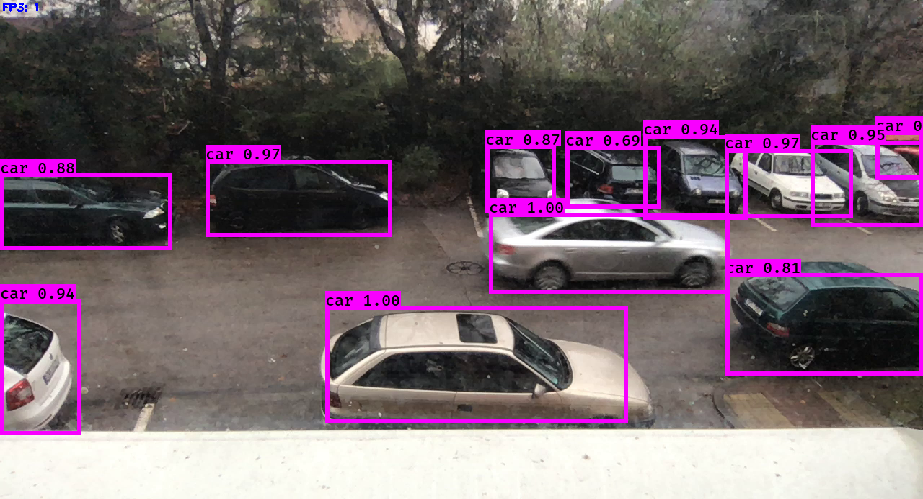
\includegraphics[width=0.90\textwidth]{imgs/yolo-np.png}
	\caption{Detection results of Mask R-CNN (top) and YOLOv3 (bottom) on 1280x720 side view footage. Source: author.}
	\label{label:comparison_np}
\end{figure}


\subsection{Stationary car detection}
The parking lot can be a frequented place with people driving around looking for a place to park, giving a right of way and many more scenarios could be happening right in the field of view of the camera. The camera footage is being ingested one frame (image) at the time in a certain period. Determining if object is stationary or not is almost impossible from a single frame\footnote{Indications of moving object in an image could be a blur, however this isn't a reliable occurence and depends on other variables like camera sensor and its settings.}.\\

In order to figure out whether car is moving or not a number of sequential frames have to be taken into consideration. Feeding these images into an object detector, extract bounding boxes of cars and compare the changes in the subsequent results. Regions that have been subsequently detected, while allowing slight variation to filter out the detector imperfections, can be considered as stationary cars.

\section{Classification of a detected parking spot}
For this chapter it is assumed that locations of the parking spots on a parking lot are known and described by axis aligned bounding boxes. These spots need to be evaluated periodically on the latest camera frames in order to get recent occupancy status of the parking lot.\\





\subsection{Datasets}
Several datasets for parking spot classification are compiled and made available for public use. Each dataset contains cropped images of parking spaces, both occupied and vacant. Each image was correctly labeled by the authors manually.
\subsubsection{CNR Parking Dataset}
CNR parking dataset is composed of 145 000 cropped images (patches) with labels taken from 9 cameras. The labels indicate whether the parking space captured in the patch is occupied or vacant. The label is  either equal to 1 for occupied spot or equal to 0 for vacant spot. The patches also have information indicating what weather type the original image was taken in (rainy, sunny, overcast). Each patch image has resolution of 150 x 150 pixels. The images can also contain a partial occlusion of tree leaves, street lamps, etc. The ratio of vacant to occupied spots is 45.3 \% / 54.7 \% in this dataset. The source parking lot is located at a CNR Research Area in Pisa, Italy. Example images from the dataset can be seen in Figure \ref{label:cnr_dataset_exampls}. \cite{cit:cnr_dataset}.
\begin{figure}[ht]
	\centering
	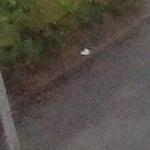
\includegraphics[width=0.45\textwidth]{imgs/cnr-vacant.jpg}
	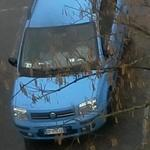
\includegraphics[width=0.45\textwidth]{imgs/cnr-occupied.jpg}
	\caption{Examples of vacant and occupied parking spots in rainy weather. Taken from CNR dataset \cite{cit:cnr_dataset}.}
	\label{label:cnr_dataset_exampls}
\end{figure}

\subsubsection{PKLot}
PKLot is another available dataset that also provides cropped images with labels. The patches have different sizes and aspect ratios. The images were captured on two different parking lots and also in the same weather scenarios as the CNR dataset. The original images were taken at Federal University of Parana, Brazil.\\

The original parking lot, where the images were taken at, has its parking spots angled at 45 degrees and authors picked only the valid parking spaces (those delimited by road markings), that can be seen in Figure \ref{label:pk_lot_orig}. The skewed segmented parking spaces were normalized into 0 degree rotation, that can be seen in Figure \ref{label:pk_lot_skew}. The dataset is also slightly imbalanced with 48.54\% patches occupied and 51.46\% vacant \cite{pklot_dataset}.

\begin{figure}[ht]
	\centering
	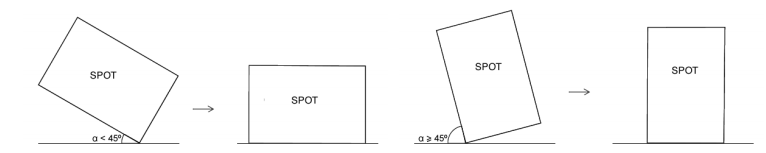
\includegraphics[width=0.9\textwidth]{imgs/pklot-skew.png}
	\caption{Skew adjustments done in PKLot dataset \cite{pklot_dataset}.}
	\label{label:pk_lot_skew}
\end{figure}

\begin{figure}[ht]
	\centering
	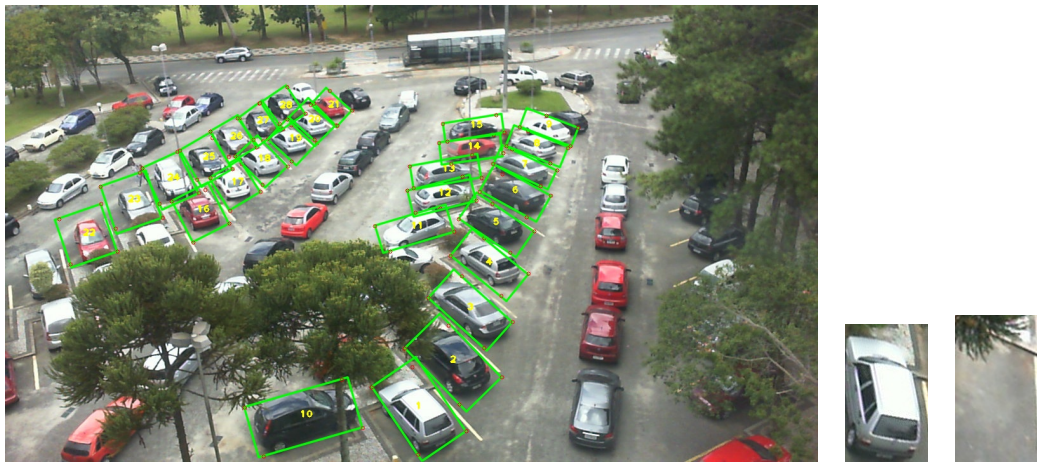
\includegraphics[width=0.9\textwidth]{imgs/pklot-example.png}
	\caption{Original source parking lot for PKLot dataset with skew adjustment example \cite{pklot_dataset}.}
	\label{label:pk_lot_orig}
\end{figure}

\subsection{Deep learning libraries}
The deep learning approach for machine learning is quickly becoming popular and many deep learning frameworks are being developed. The libraries often abstract the mathematical apparatus used for training the network and provide straight forward way to design the network models. Some of the most prominent libraries are compared in the following sections.

\subsubsection{Caffe}
Caffe is a deep learning toolkit for training, testing and deployment developed by Berkeley AI Research (BAIR). It is written in C++ language and it is one of the most mature implementations. It supports running computations on both CPU and GPU\footnote{The most deep learning frameworks only support Nvidia video cards and their CUDA framework.}. Caffe also provides a Python interface to interact with the library \cite{cit:mltoolkits}. 

\subsubsection{Tensorflow}
Tensorflow is an open source platform for machine learning developed by Google. The library is written in C++ language in order to support multiple computer architectures. Enabling mobile devices and websites to utilize Tensorflow for machine learning applications. It also supports multiple GPUs, CPUs and TPUs (Tensor Processing Unit). TPU is a custom ASIC based hardware for deep learning computations. Tensorflow is one of the most adapted framework for deep learning \cite{cit:tensorflow}.

\subsubsection{Deeplearning4j}
Deeplearning4j is an open source deep learning library for the JVM\footnote{Java Virtual Machine} written in Java and Scala. The library takes advantage of Apache Spark and Hadoop for distributed CPU and GPU computation. Official documentation claims the performance to be equal to Caffe described above. 
\subsubsection{Keras}
Keras is a high-level API written in Python that was designed to allow fast prototyping and make the process of experimenting and developing faster and more friendly overall. The library itself relies on underlying backends such as Tensorflow. Recently it became a part of the official Tensorflow release. Together they are the most adapter framework for deep learning \cite{cit:keras}.

\subsection{Model of the network}
The authors of CNR parking dataset already experimented with training mAlexNet and mLeNet models using Caffe framework. The \textit{m-} prefix stands for \textit{mini} - meaning it is a reduced version of the original model. The authors chose this model because they were deploying the network to a Raspberry Pi computer with limited resources. The resulting inference time for 50 parking spots was around 15 seconds. \cite{cit:cnrparkclassification}.

\section{Ingesting camera feed}
Due to the lack of actual parking lot camera, an attempt was made to create custom one using Raspberry Pi Zero W mini computer and an accessory camera.

Raspberry Pi Zero W offers 1GHz single core CPU, 512 MB RAM and Bluetooth 4 + Wi-Fi 2.4GHz functionality. Its low power consumption allows it to run off of a 10 400 mAH powerbank for around 3 days with the camera running. The camera is 1.3 Mpx capable of capturing full HD images (1920x1080) at 30 FPS. Setup can be seen in Figure \ref{label:raspiwithcam}.\\

The Raspberry Pi operating system Raspbian has already prebuild tool for controlling the camera called \texttt{raspivid}. Running the stream is as simple as running the command below. The tool interacts with the camera hardware and the output is piped into VLC media player in order to create a RTSP stream. 

\begin{minted}[breaklines]{bash}
raspivid -o - -t 0 -w 960 -h 540 | cvlc -vvv stream:///dev/stdin --sout '#rtp{sdp=rtsp://:8554/}' :demux=h264
\end{minted}


\begin{figure}[ht]
	\centering
	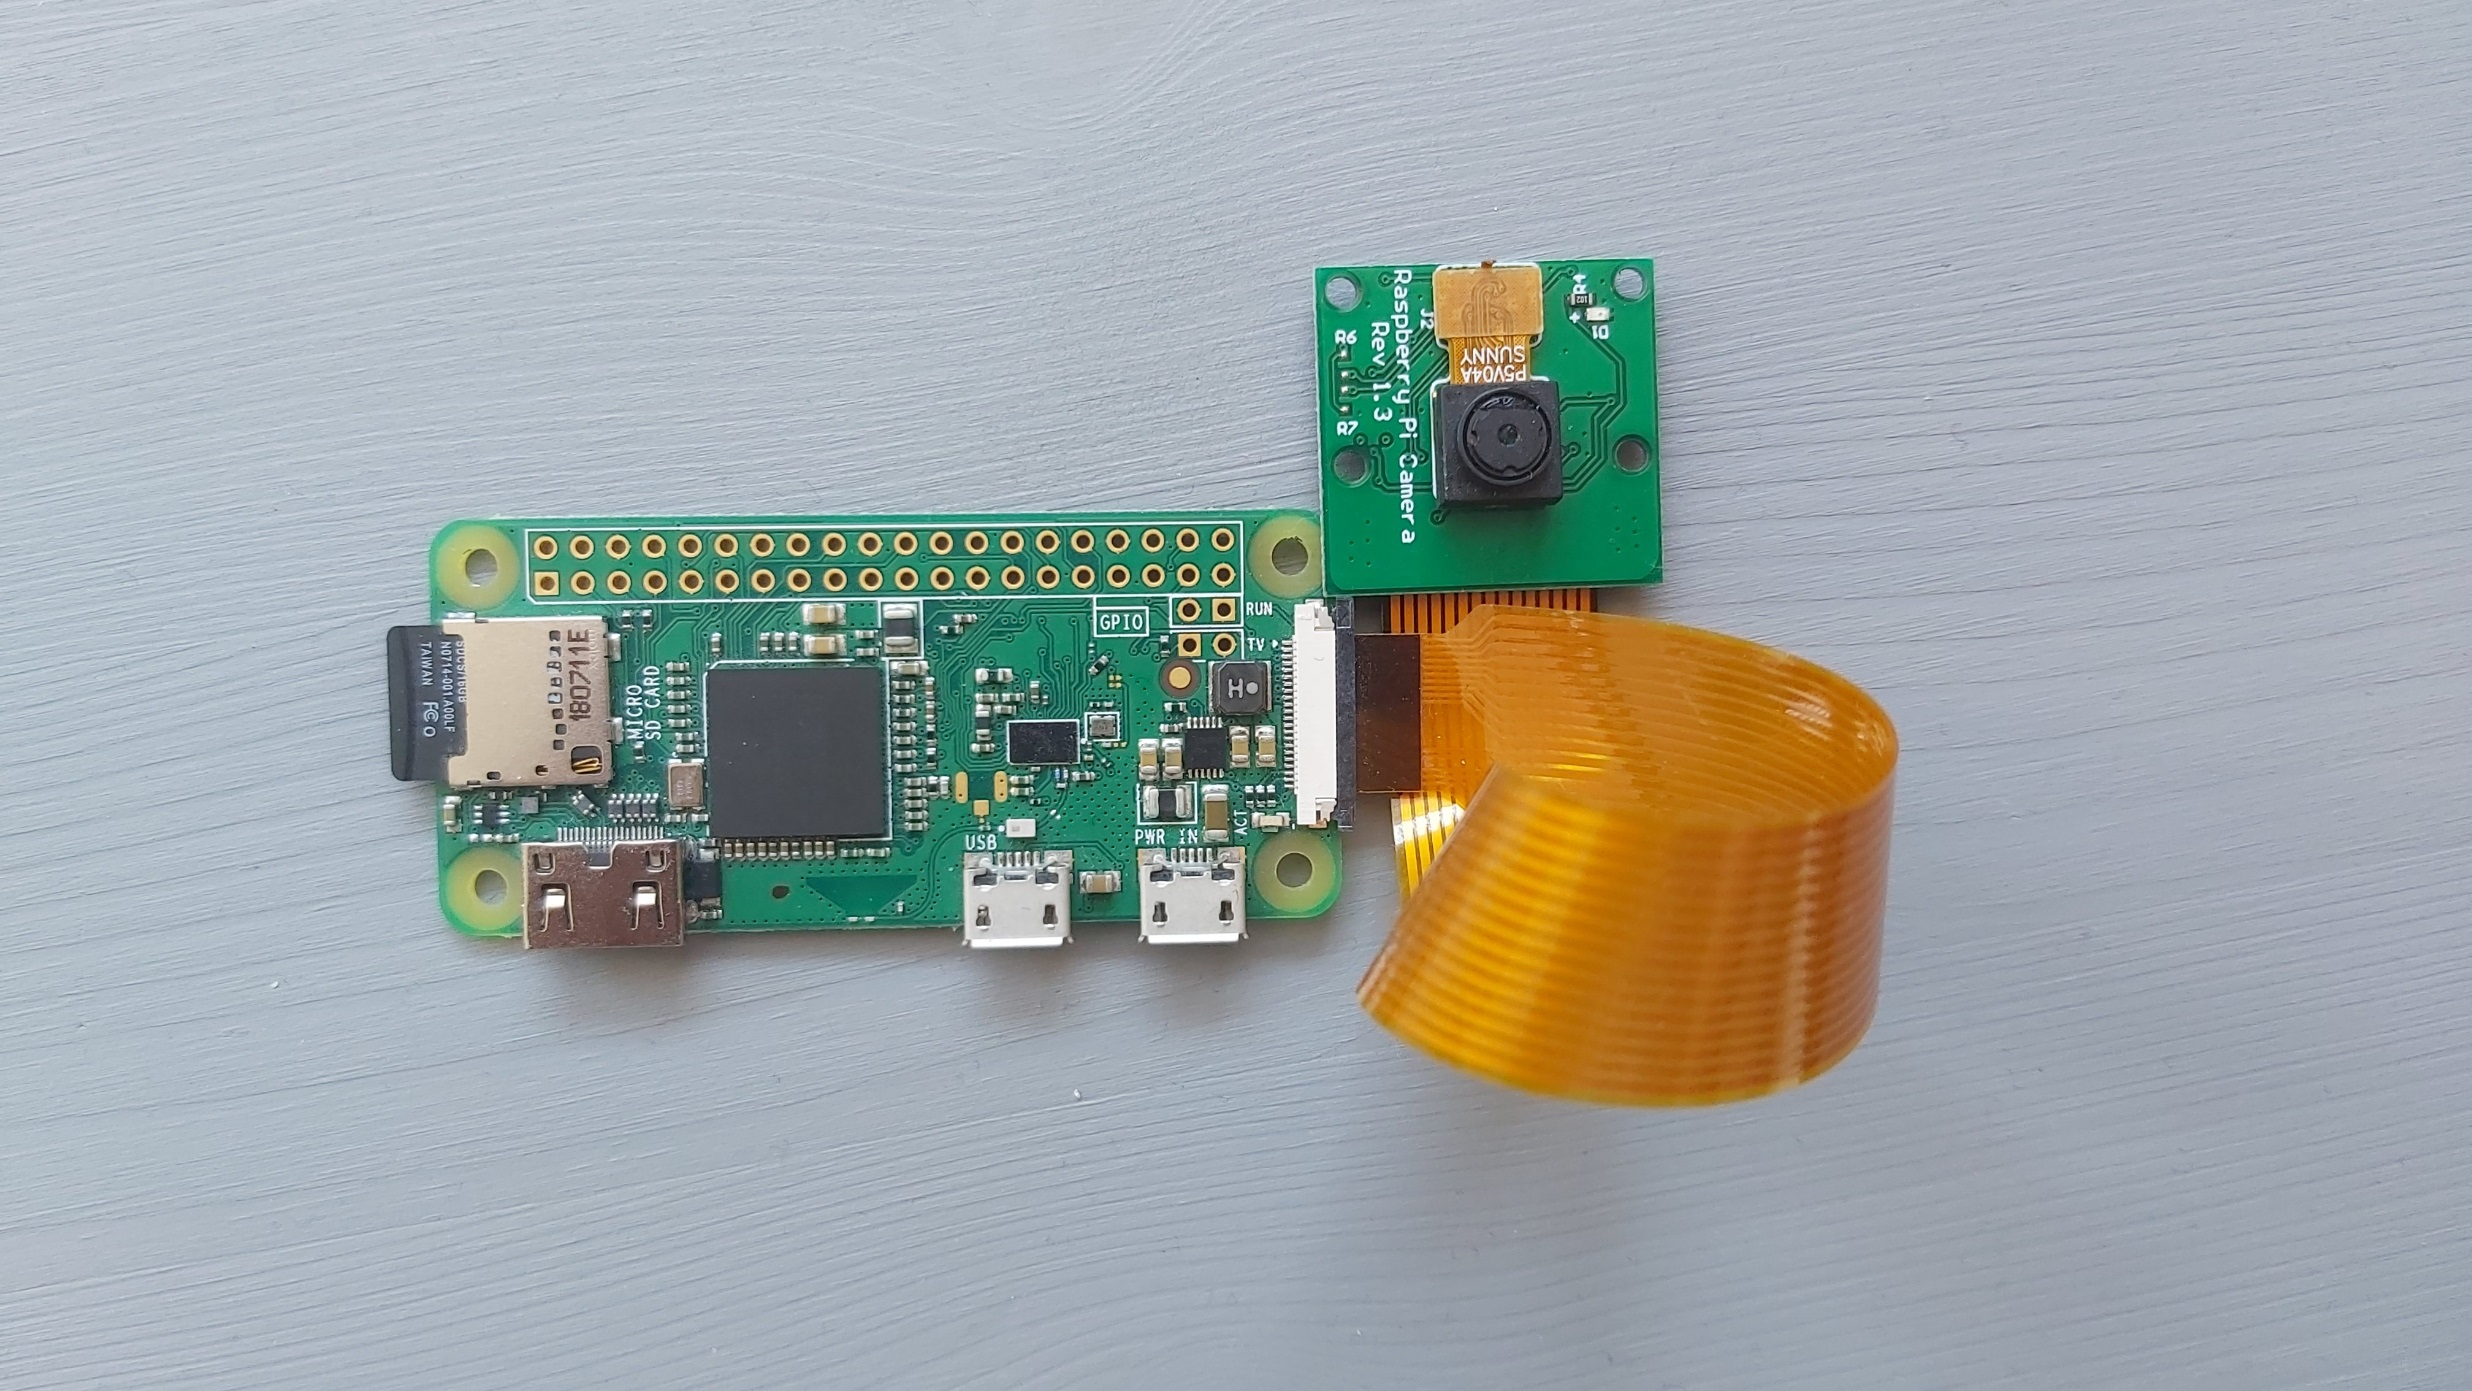
\includegraphics[width=0.9\textwidth]{imgs/custom-ipcamera.jpg}
	\caption{Raspberry Pi Zero W with 1.3 Mpx camera attached. Source:
	author.}
	\label{label:raspiwithcam}
\end{figure}
\subsection{RTP}
Real-time Transport Protocol provides end-to-end transport of real-time multimedia over the network. The protocol itself is agnostic to underlying network transport layers, but it relies on underlying protocol to provide demultiplexing of the data (most often UDP).\\ RTP is intended to be used along with RTCP (Real-time Transport Control Protocol) which provides quality of service (QoS) feedback and session management \cite{jain-rtp}.

\subsection{RTSP}
Real-time Transport Streaming Protocol is an application layer protocol used to control the delivery of real-time streaming multimedia. Original RFC7826 document describing RTSP says: \enquote{RTSP acts as a
"network remote control" for multimedia servers.} \cite{rtsp-rfc}. It supports functionalities like play, pause, stop, etc. RTSP is agnostic to the underlying protocol that handles the data delivery. For example, it can use RTP, UDP or TCP.

\section{Containerization and Virtualization}
Containerization\footnote{Other terms than container are also used in this regard: zone, partition, virtual kernel, jail. } is a concept that originates from operating system level virtualization. Kernel of such operating system allows the existence of isolated user spaces (containers). A program running in an isolation can only access resources that have been assigned and allocated to the container via control groups.\\

Virtualization uses abstraction of physical hardware and hypervisor in order to run multiple fully fledged operating systems on top of the host operating system. One instance of such abstraction is called a virtual machine. \\

Container is also suitable only for running one main process at the time and the containers life is tightly bound to the life of the process. When the process is finished, the container is no longer running. Whereas the virtual machine behaves just like ordinary computer running an operating system.



\subsection{Docker}
Docker is a container virtualization implementation. Under the hood it uses Linux kernel features to sandbox processes. The original idea is to package software and its dependencies into one container and the host machine is able to run multitude of such containers in an isolation.\\

The Docker solution is native to Linux operating systems where the kernel contains all the necessary system functions to support containers. However, Docker is also available to macOS and Windows. Running on macOS and Windows is achieved by using a read-only Linux virtual machine, created during installation, that actually hosts the containers. Windows 10\footnote{Only applicable for Enteprise and Professional versions.} and Windows Server 2016+ do additionally offer native support Windows containers. Linux and Windows container are not compatible with each other in general and only one type of them can be run at the same time in the Docker environment. \\

Docker gained a lot of popularity and is becoming the industry leader in the field. It is available on all major operating systems  like Windows, macOS and Linux and is adapted by notorious big tech companies such as Google, Microsoft and Amazon. For example, in their respective cloud services. \\

Container uses significantly less disk space, has faster boot time and less overhead than a virtual machine \cite{docker-performance}.


\begin{figure}[ht!]
	\centering
	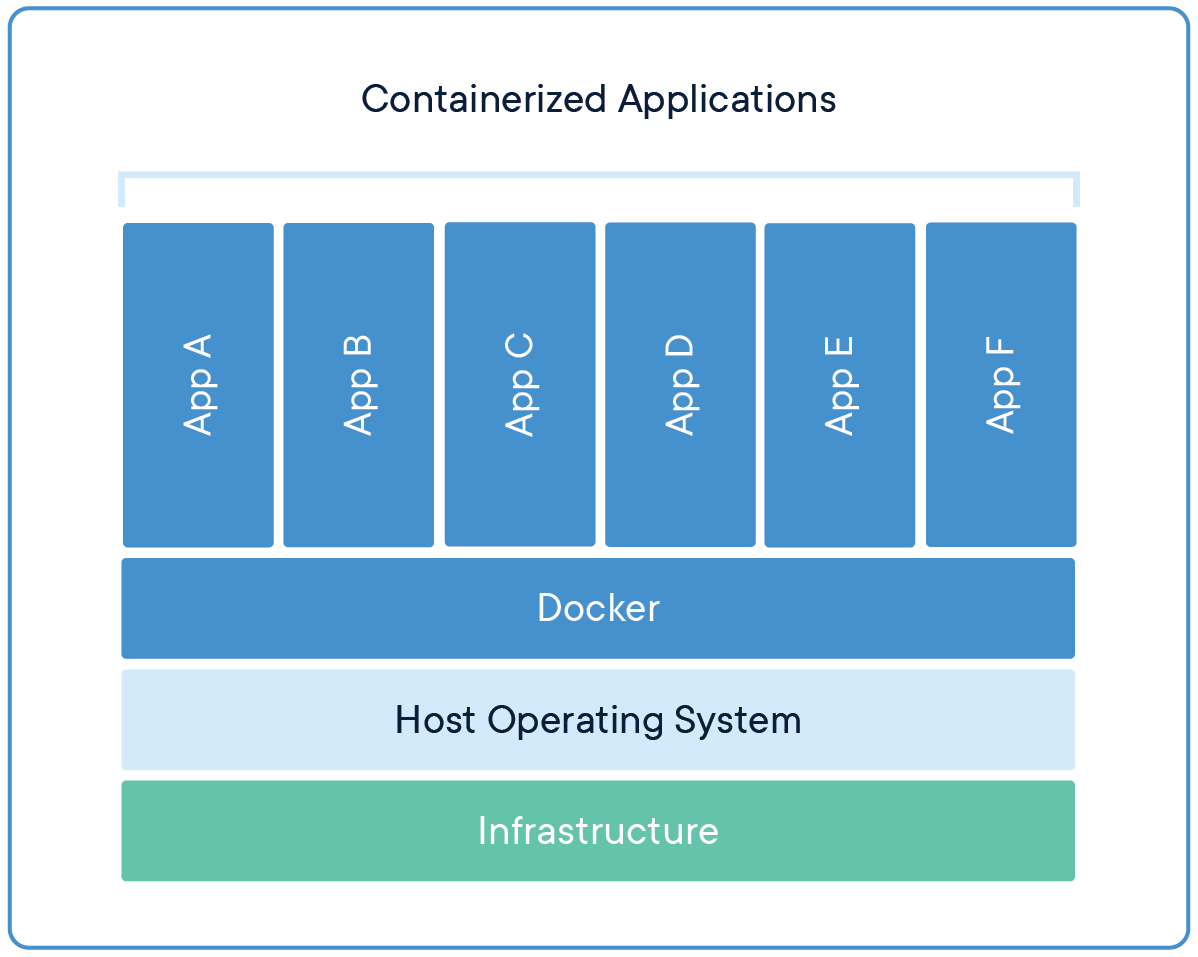
\includegraphics[width=0.45\textwidth]{imgs/docker-stack.png}
	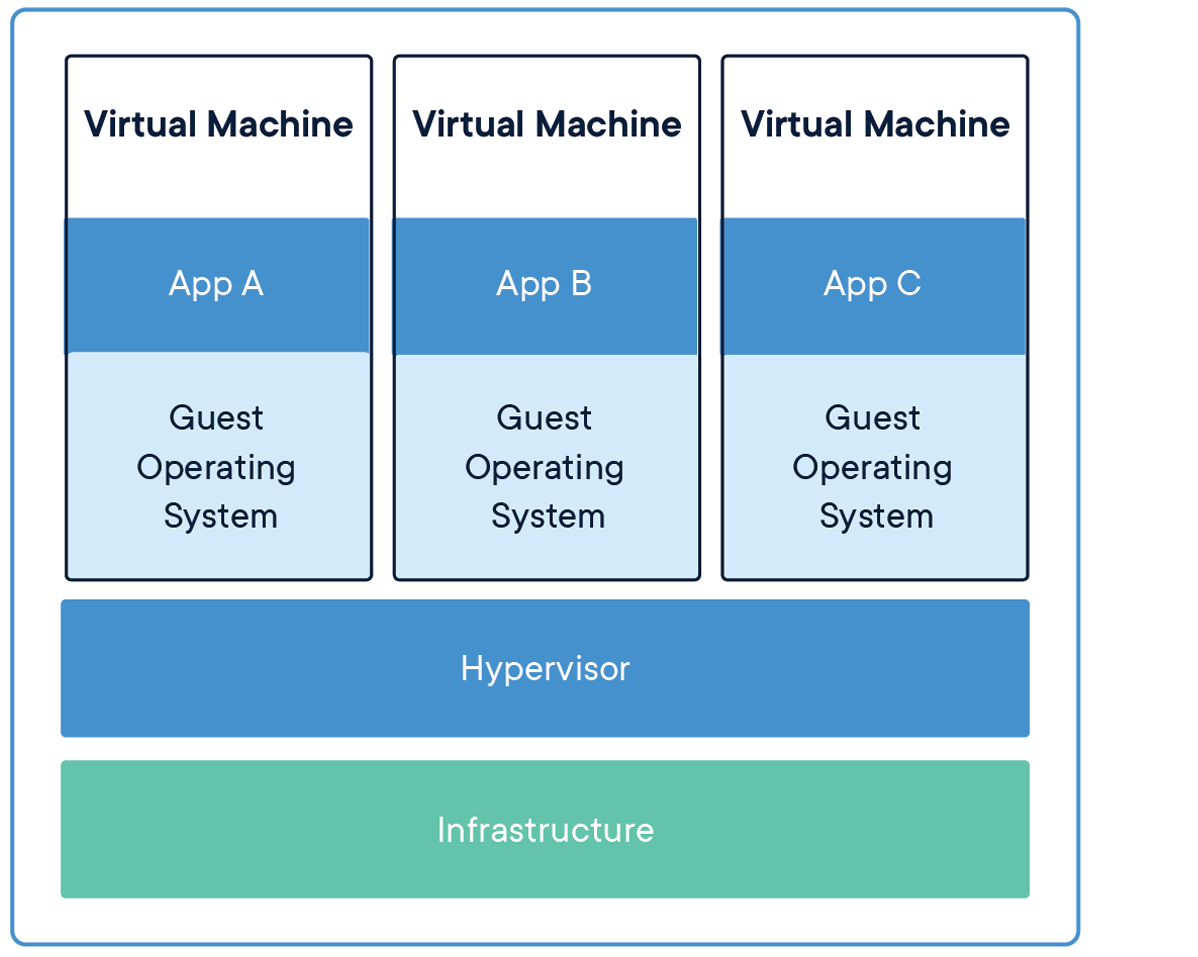
\includegraphics[width=0.45\textwidth]{imgs/vm-stack.png}
	\caption{Comparison of container stack and virtual machine stack.}
	\label{label:containervsvm}
\end{figure}

\subsection{Containerizing object detectors}
Above mentioned object detectors and their implementations come with a lot dependencies that are not necessarily compatible or the dependency versions are deprecated\footnote{For example, Tensorflow libraries because of the very fast development in the field of deep learning.}. Containerization of the object detector can be very effective way of dealing with such inconsistencies and could also streamline multiple deployments if needed. However, there are caveats in utilizing GPU for the object detectors in containers. The problem is that CUDA framework by NVIDIA, used by deep learning frameworks,  is supported only for containers running on Linux host system. \\

\subsection{Development advantages}
Docker has also build an ecosystem around itself.  It is called Docker Hub and it provides thousands of premade images for different applications which can be easily and reproducibly ran across platforms. \\



\chapter{Design}

\section{Use Cases}
The following is a description of use cases from users perspective. The use case diagram may be seen in Figure \ref{label:uc_diagram}.


\begin{figure}[ht!]
	\centering
	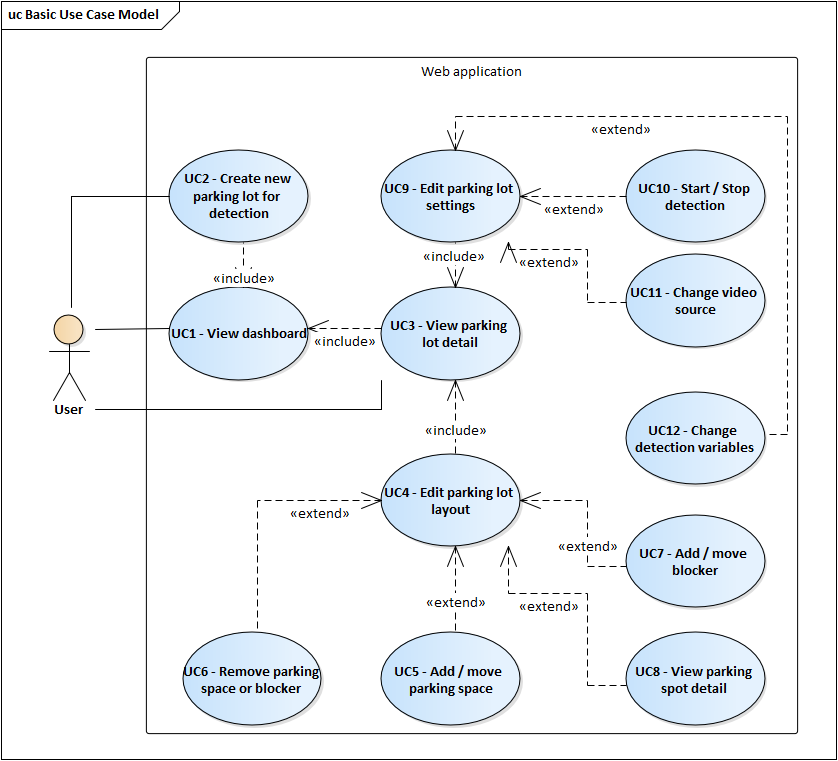
\includegraphics[width=\textwidth]{imgs/uc-diagram.png}
	\caption{Diagram of use cases.}
	\label{label:uc_diagram}
\end{figure}

\begin{description}
    \item [UC1 - View dashboard] An overview of all parking spots managed by the application is displayed along side with brief information, such as recent photo of the parking lot and occupancy status.
    
    \item[UC2 - Create new parking lot for detection] 
    The dashboard view in use case \textbf{UC1} also allows the user to create a new parking lot for detection. The user is presented with simple form to fill out the required information, such as the name of the parking lot and video source URI.
    
    \item [UC3 - View parking lot detail]
    The user can select a parking lot from dashboard \textbf{UC1} in order to see all the information about the parking lot, such as current occupancy, occupancy history and image of the parking lot with visualized layout of detected parking spots and blockers.
    
    \item[UC4 - Edit parking lot layout]
    The lot layout is displayed in parking lot detail \textbf{UC3}. The user can manipulate the existing layout or create a new one.
    
    \item[UC5 - Add / move parking space]
    The user can add a new parking space (rectangular delimiter) into the layout. Existing parking space can be freely moved and resized for the optimal coverage of the actual parking space.
    
    \item[UC7 - Add / move blocker]
    Blocker delimiter can be added and be manipulated in the same way as parking spot. Blocker restricts the covered area from object detection.
    
    \item[UC6 - Remove parking space or blocker]
    Each delimiter, either parking spot or blocker, can be completely removed from the layout.
    
    \item[UC8 - View parking spot detail]
    For every highlighted parking spot a detailed history of its occupancy can be displayed.
    
    \item[UC9 - Edit parking lot settings]
    Settings of the parking lot detection can be accessed from the parking lot detail \textbf{UC3}.
    
    \item[UC10 - Start / Stop detection]
    The detection pipeline for individual parking lots can be toggled on or off in the lot settings \textbf{UC9}.
    
    \item [UC11 - Changing video source]
    The source URI of the video stream can be changed in the settings of the parking lot.
    
    \item[UC12 - Change detection variables]
    The user can adjust other variables to smoothen or troubleshoot the detection if there is an issue.
    
    
    \end{description}

\section{Application Services}
Each part of the application process mentioned in previous chapter has its own specific needs and characteristics and the final architecture should reflect that in order to achieve good performance and scalability. For example, the object detectors performance heavily relies on the hardware it is being run on, more specifically the GPU card. On the other hand the camera ingestion software needs to provide an actual image every fixed amount of frames, but it is possible that more than one instance of the camera ingestion service is running at the same time. \\

The functionalities are divided into services (separate applications).

\section{Services}
\subsection{Slicers}
Slicer is responsible for consuming the camera output and extracting a single frame (image) at well defined frequency as output. The extracted image is then propagated for further processing.\\

There is a new slicer for every parking lot currently being processed. The reason for it is to avoid problems with the stream capture, such as latency or network errors, which could lead to a failure to deliver a new frame for every parking lot if the slicer was shared for multiple parking lots. \\

Each instance of slicer is managed by manager that handles restarting of the slicers in case of error or stopping the slicers on users request.
\subsection{Detector}
This service takes the image captured from the camera by slicer and performs object detection on the image. The detection is achieved utilizing already trained deep learning based object detector. The locations defined by bounding boxes, that were classified as vehicles, are then passed down further to the pipeline.

\subsection{Spotter}
Spotter takes in the extracted locations of the vehicles produced by the detector and performs time based evaluation on the data in order to filter out moving vehicles and other unwanted occurrences that can be present in the detection. Spotter acknowledges or denies the proposed locations based on the evaluation, leading to the approximate location of the actual parking spot.\\

Spotter stores the actual state of the parking lot, namely the locations of the spots and their statuses extracted from the incoming information, in the database. \\

This service also separately listens for the messages from the slicers and periodically passes the most recent image with corresponding accepted parking spots and sends them to a classifier for evaluation. The response from classifier is then also processed and stored in the database.
\subsection{Classifier}
Classifier listens for requests made by Spotter. The request contains the locations of the acknowledged parking spots and corresponding image they should be classified on. Each location of the parking spots is cropped from the image and then classified. The classified parking spots are then sent back to the Spotter.

\subsection{Backend}
Backend is a central service responsible for orchestrating the whole pipeline. This component handles Slicer initialization in order to begin analyzing the camera footage. Maintains the connection with the database. Also provides the information about the parking lots and parking spots and allows the control of the pipeline via exposed REST API. This particular component is meant to be a singleton per single deployment of whole application.


\section{Communication of the components}
There is a couple assumptions to be made about the data sent in messages between the services. Some of the messages contain a raw image representation, directly affecting its size. Not every service needs to be present in the pipeline, for example the object detector once all the parking spots are detected or the user opted out for filling out the parking spot locations manually. More than one service can be dependent on data produced by other service. The communication system should keep a low overhead in order to keep up with the real-time nature. Additionally, more than one instance of a single service type can be running. \\

To ensure scalability and to meet assumed needs a producer-consumer approach is used. Essentially every data message produced is a work impulse for another service which can yield another data message upon its completion. For the actual message handling and delivery a message broker is used, ultimately decoupling the components and preventing the instances to be directly tied together.\\

A communication diagram, that may be seen in Figure \ref{label:communication_diagram}, gives a brief overview how the services are communicating.


\begin{figure}[ht!]
	\centering
	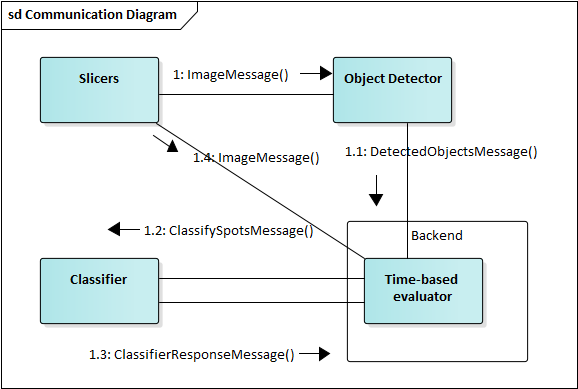
\includegraphics[width=\textwidth]{imgs/comm-diagram.png}
	\caption{Communication diagram of the described services.}
	\label{label:communication_diagram}
\end{figure}

\section{Communication middleware}
Messaging is divided into two primary concepts. First one is a producer-consumer and the second is publisher-subscriber. In producer-consumer approach the messages from producers are distributed across consumers. In publisher-subscriber the message is broadcasted to all subscribers\\

In this section, implementations of data handling (messaging) solutions are compared.

\subsection{RabbitMQ}
RabbitMQ is originally an open source implementation of AMQP (asynchronous message queuing protocol) which is business standard for passing messages between applications focused on reliable transmit. Currently supports also MQTT, HTTP and Websockets. RabbitMQ supports both approaches of message handling via push or poll mechanics. When using push method the consumer or subscribed gets notified about new message, using pull approach the consumer has to check for new message \cite{cit:rabbitmq} \cite{cit:kafkavsrabbit}.
\subsection{Apache Kafka}
Kafka is an open source distributed streaming platform developed at LinkedIn. Kafka divides the data into topics which are further divided into partitions. Each partition has an immutable, ordered and durably persisted data records. Producers send byte data into topics and consumer groups are polling the topic for the record. If the consumers are in the same group then the messages from a topic are load-balanced across them. Otherwise a consumer gets a copy of the message in each distinct group. Kafka regards the topic as a stream of records. The records are guaranteed to be in order in a partition. Kafka can support both concepts of messaging described above \cite{cit:kafkavsrabbit} \cite{cit:kafka}.

\subsection{Comparison}
When choosing an implementation a key trade-off has to be made between ability to handle very high throughput and reliability of the delivery. Apache Kafka is able to achieve high throughput due to its good cluster scaling. However, the application has to be tolerant to seldom message drops, as they might occur. RabbitMQ doesn't achieve such throughput as Kafka but it is suited to applications where reliability of the messages is more important than optimal throughput \cite{cit:kafkavsrabbit}.








\section{Database}
The processed data that are be persisted can be divided into two types. First being the actual data about a parking lot, for example the location of parking spots, current occupancy status and it's settings. The second kind is the historical data gathered as the application runs in order to evaluate the status of the parking lot over time. A single relational database is used to hold all the information about all the parking lots being monitored by the application. The proposed data structure can be seen in Figure \ref{label:domain_model}.\\


The root of the structure is a \texttt{Lot} object, which holds static information, such as the name that user specifies along with settings that will determine the URI of the camera source, how often a snapshot from the camera should be taken and time that is needed for a parking spot to be acknowledged.\\

\texttt{Lot} is composed of \texttt{ParkingSpot} objects that hold information about a single parking spot in a frame such as its location in the image, its status whether it is acknowledged or pending and \texttt{TTL} (Time to live) indicating the parking spots progress to be acknowledged.\\

The designated objects to track histories of both the parking lot and the parking spots hold occupancy statuses valid for it's associated timestamp. Ultimately, the most recent entry in the history is to be considered the actual status of the lot or spot.






\begin{figure}[ht!]
	\centering
	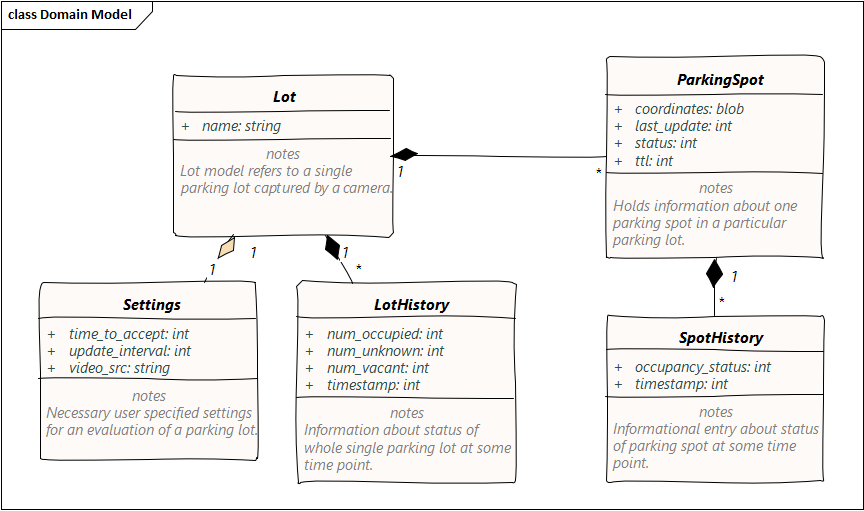
\includegraphics[width=\textwidth]{imgs/domainmodel.png}
	\caption{Domain model diagram describing relationships between persisted data.}
	\label{label:domain_model}
\end{figure}

\section{Web User Interface}
The main entry point for the user is web based application. Also referred to as frontend in this work. Its job is to consume the REST API provided by backend and present the data in a human friendly way.

\subsection{Dashboard}
The dashboard is a landing page of the application. The page lists all available parking lots currently being processed and provides information about how many spots are occupied or vacant. \\

Dashboard also allows to setup a new parking lot. Clicking on the existing parking lot will take the user to the parking lot detail. Wireframe diagram of the dashboard can be seen in Figure \ref{label:dashboard_diagram}.\\

The page for adding a new parking lot is just a simple form where user specifies the name of the lot and the video source URI.

\begin{figure}[ht!]
	\centering
	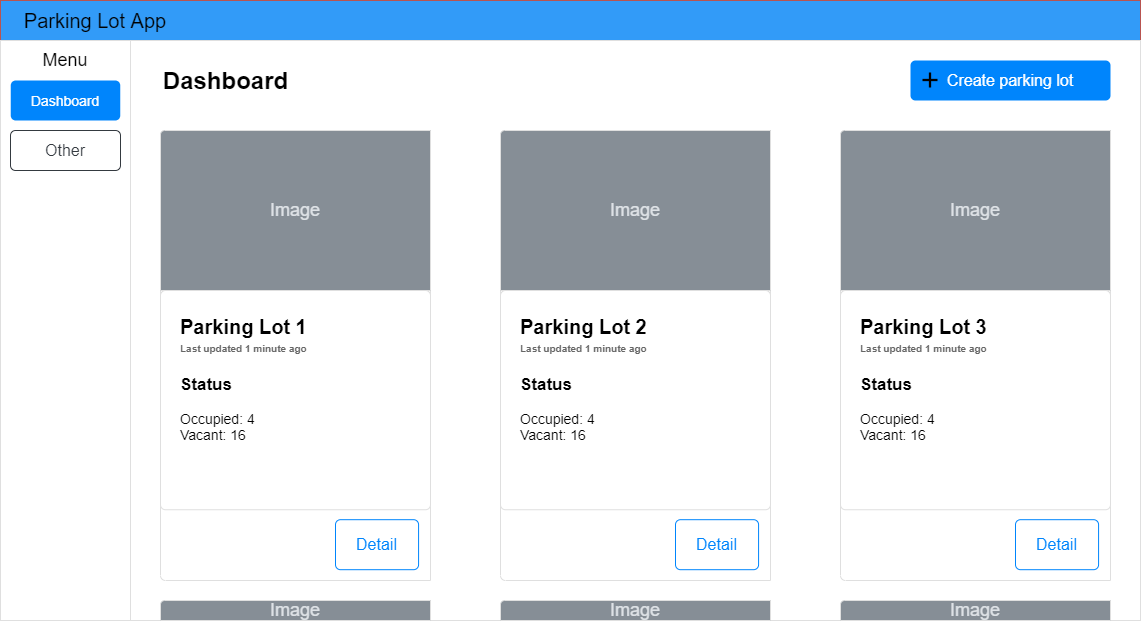
\includegraphics[scale=0.5, angle=90]{imgs/dashboard-wireframe2.png}
	\caption{Wireframe diagram of the dashboard page.}
	\label{label:dashboard_diagram}
\end{figure}
\subsection{Parking lot detail}
This page provides the history of occupancy, current status and allows to manipulate the detection settings. It also provides the most recent camera snapshot with current detected and accepted parking spot and blocker rectangles rendered onto. Blocker rectangles are only placeable by the user and any detection located in the blocker area is omitted from further processing.\\

The rectangles can be manipulated in following manner by the user:

\begin{description}
    \item [Highlight] When clicked on, the rectangle will become highlighted and the user can perform following actions.
    \item [Translation] Any highlighted rectangle can be repositioned using drag and drop mechanic.
    \item [Scale] Highlighted rectangle has anchors displayed around its border. Allowing the user to change the scale and aspect ratio of the rectangle.
    \item [Add a parking spot] Add a new rectangle indicating an accepted parking spot.
    \item [Add a blocker] Add a new rectangle that excludes the area contained by the rectangle from detection.
    \item [Delete the rectangle] Any highlighted rectangle can be deleted.
\end{description}

This gives user the ability to intervene and rectify incorrect or otherwise malformed parking spot detections. The user can also skip the automatic detection of parking spots and define own bounding boxes entirely. This feature can be useful when for example the environment renders the detector unusable or there is an absence of computing power to do the detection. The wireframe model can be seen in Figure \ref{label:detail_diagram}.\\

Once a rectangle is highlighted the user can click on a button to see the detail of the parking spot marked by the rectangle. The detail shows the occupancy history of the parking spot along with its actual state.

The settings wireframe can be seen in Figure \ref{label:settings_diagram}. It allows the user to tweak the processing constants like TTL of the spots to adjust the detection behavior.


\subsection{Mobile layouts}
The layouts for mobiles, tablets and other portable devices with smaller screens are very similar to the desktop. The contents overflowing the width of the screen are going to be stacked vertically to fit the screen. This is known as column-drop. The main menu is implemented as sliding side menu that can be opened by clicking the top menu icon. The same applies for the settings side menu in the parking lot detail.\\

Also manipulating rectangles of the parking lot will be disabled on small devices, since the lack of pointer precision and screen size may lead to bad user experience.




\begin{figure}[ht!]
	\centering
	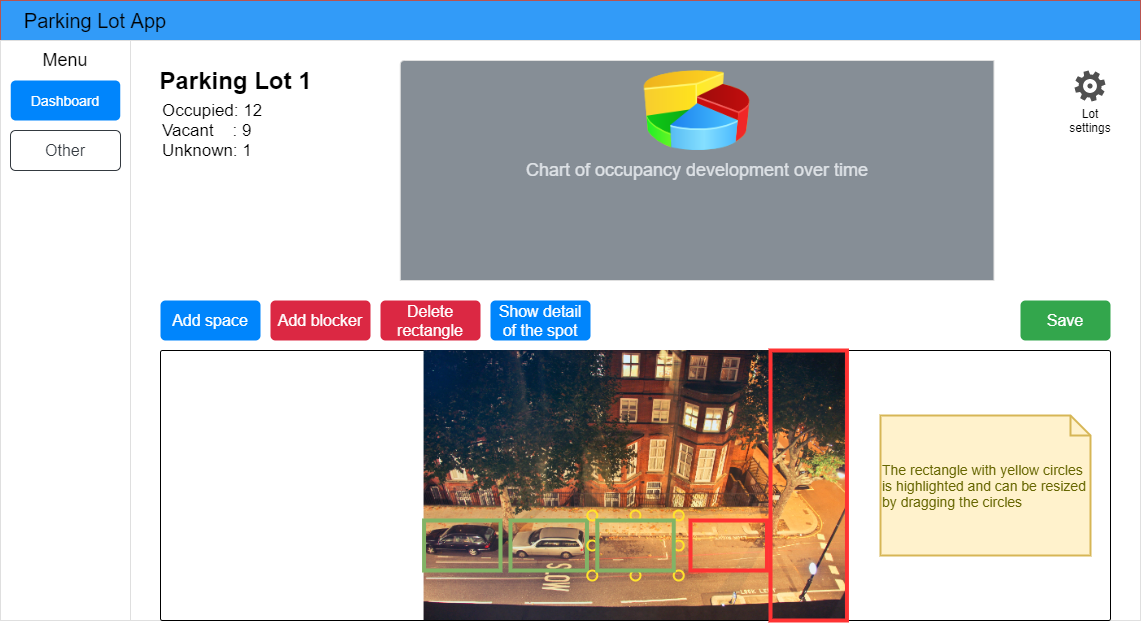
\includegraphics[scale=0.5, angle=90]{imgs/wf-detail.png}
	\caption{Wireframe diagram of the parking lot detail page.}
	\label{label:detail_diagram}
\end{figure}

\begin{figure}[ht!]
	\centering
	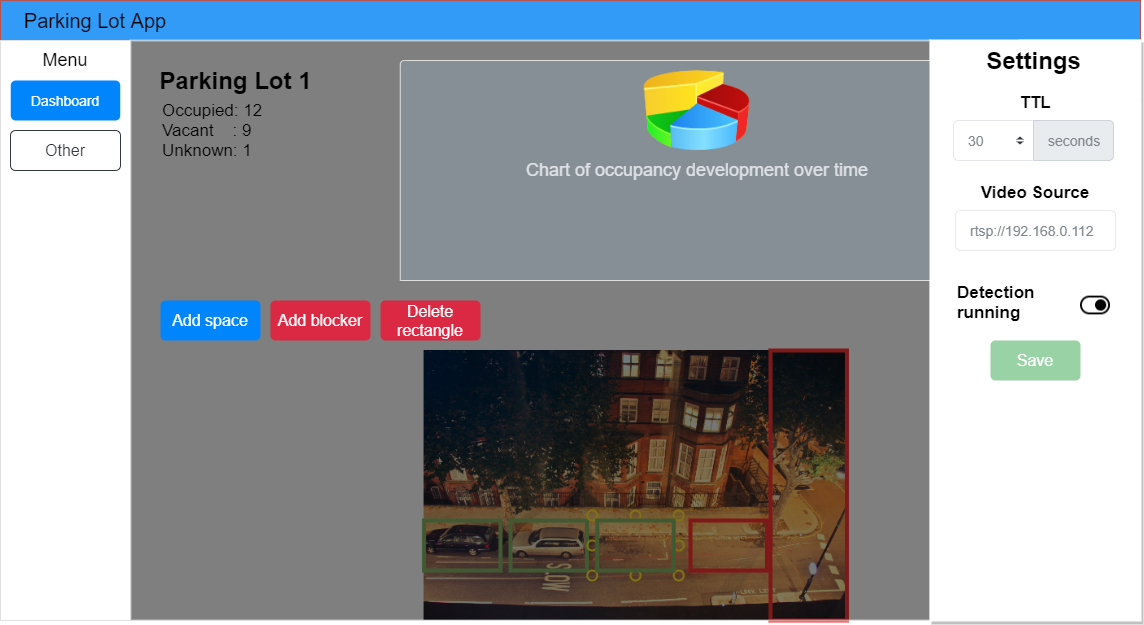
\includegraphics[scale=0.5, angle=90]{imgs/wf-settings.png}
	\caption{Wireframe diagram of the settings in the parking lot detail page.}
	\label{label:settings_diagram}
\end{figure}

\begin{figure}[ht!]
	\centering
	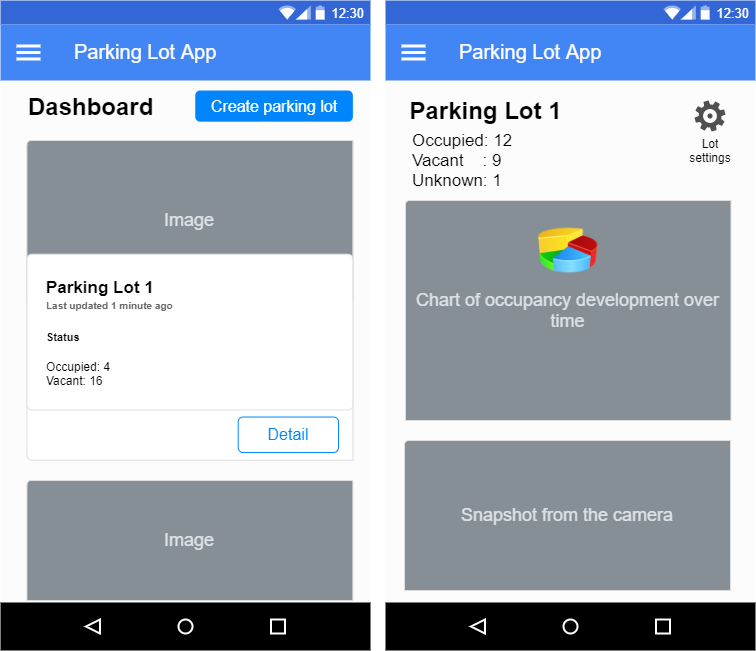
\includegraphics[scale=0.5]{imgs/wf-mobile.png}
	\caption{Mobile version wireframes of the Dashboard on the left and parking lot detail on the right.}
	\label{label:diagram_mobile}
\end{figure}

\section{Classifier}
The classifiers input is a cropped rectangular region from the original image containing a single parking spot. The rectangle delimiting a parking spot will not always have the same dimensions, it will vary according to the angle, distance and height of the camera. However, the classifier will always expect the input to have the same dimensions. \\

This is going to be addressed using resizing. If the cropped image is smaller than the required dimension an artificial padding is going to be added. In case the cropped image is bigger it will simply be scaled down to fit.\\

The cropped image is going to be classified and naturally resulting into one of two classes - vacant or occupied. The output of the neural network is going to be vector indicating the probabilities of both classes. The class that scored higher probability is chosen as the result.

























\chapter{Implementation}
This chapter describes the implementation of the services and applications parts described in the previous chapter and introduces used frameworks and libraries. All of the pipeline services are written in Python language.\\

Python is an interpreted, high-level, object-oriented programming language widely used for both scientific computing and software development. Large amount of scientific libraries are available in Python via wrappers, while using underlying implementations in compiled languages such as C/C++ for maximizing the performance.



\section{Code repository}
The whole application development is being versioned using Git versioning system along side with GitHub service in order to preserve the history and changes of the code and also for backup. The repository is being created under the \textit{OpenDataLab's} account with GNU GPL licence and can be freely downloaded on the following URL.\\

\url{https://github.com/opendatalabcz/parking-spot-detection}

\section{Kafka integration}
The communication middleware chosen for the implementation is Apache Kafka. Kafka requires a running instance of another application called ZooKeeper in order to run itself. ZooKeeper is a service for coordination and support of distributed applications. It is also developed and maintained by Apache.\\

For the purpose of this work, two Docker containers for deploying Apache Kafka were created. One container is used for running the ZooKeeper and the second one is for running Kafka. The images used for this are both available on Docker Hub and can be found on following URLs. \\

\url{https://hub.docker.com/r/wurstmeister/kafka}\\
\url{https://hub.docker.com/r/wurstmeister/zookeeper}.\\

The advantage of using containers is the ability to spawn more brokers as containers, consistent pre-configuration of the Kafka instance (topics, ids, etc.) in the Docker file and not polluting the host system with dependencies.\\

It is good to point out that the implementations of the services described in this thesis will work with any properly configured Kafka instance, regardless of the environment it is running in.


\section{Messages}
Since every service is written in Python language. To avoid code duplication a separate code package is created and then imported by the services. One such example are the messages. Every message is a class describing the contents of the message with methods for serializing logic used by the producer when sending the message and deserializing logic used by the consumer when receiving the message. The class diagram of the messages may be seen in Figure \ref{label:messages_class_diagram}.

\begin{figure}[ht!]
	\centering
	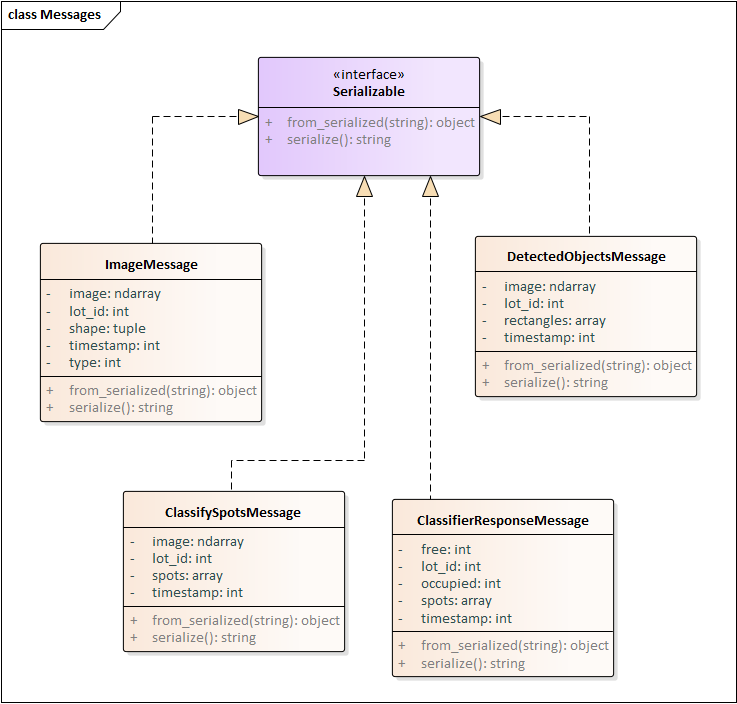
\includegraphics[width=\textwidth]{imgs/messages-class-diagram.png}
	\caption{Class diagram of messages sent by the services.}
	\label{label:messages_class_diagram}
\end{figure}







\section{Object Detector}
Existing implementation of object detector is used and adjusted, because implementing and training custom one is outside the scope of this work.\\

The detector is encapsuled in its own service. That means the whole pipeline described in the analysis is agnostic to the actual implementation of the detection engine and can be easily changed, making it a future proof design.\\

The chosen implementation of the object detector is a project called Mask RCNN\footnote{\url{https://github.com/matterport/Mask_RCNN}} developed by Matterport, Inc. The object detection model is based on Faster R-CNN described in the analysis chapter. This model was chosen because of its ability to detect more fine grained objects than YOLOv3 making it more usable for smaller regions on wider fields of view. The model is implemented in Python language and uses Keras with Tensorflow as the deep learning libraries.\\

The implementation yields consistent detection of vehicle occurences across video frames, but there is slight variation in the detected bounding boxes on subsequent video frames, even when the camera was completely stationary. This inconsistency is addressed in the Spotter component.

\section{Backend}
The core framework used to build the backend is Django\footnote{https://github.com/django/django}. Django is an open source web application framework written in Python. The framework consists of loosely coupled components and comes with Object-relational mapping (ORM), authentication, URL routing, internationalization and security features out of the box. Each Django project consists of units called \textit{apps}. App is meant to have a single responsibility. Django is also able to run Python scripts in its own context.\\

\subsection{Database}
The database is in a separate app and is created using Django ORM capabilities and it reflects the domain model designed in previous chapter.
Django officially supports following database engines: PostgreSQL, MariaDB, MySQL, Oracle, SQLite and there are also third party plugins extending the support. Django uses model classes defined in \texttt{models.py} file inside app in to order to fabricate migration files. Each migration file corresponds to a change in a database. Migrations are converted into native database machine SQL and applied in chronological order, providing versioning, database history and option for rollback.\\

The database engine used for this project is PostgreSQL. The database itself is setup to be running in a Docker container using official PostgreSQL image available on Docker Hub\footnote{\url{https://hub.docker.com/_/postgres}}. It is a very elegant solution deployment and development wise and it doesn't interfere with present installation of the database engine, should there be any. Backend can be pointed to use any PostgreSQL instance if Docker container is not desired.\\


There is also a Docker container with PostgreSQL admin web application for easy inspection of the running database.\\


The actual created database model inside the PostgreSQL by Django ORM can be seen in Figure \ref{label:relational_model}.\\

\begin{figure}[ht!]
	\centering
	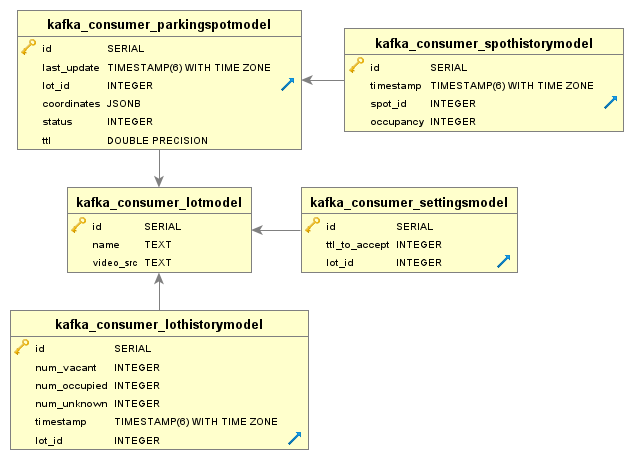
\includegraphics[width=\textwidth]{imgs/parkschema2.png}
	\caption{Relational model of the database entities.}
	\label{label:relational_model}
\end{figure}

The coordinates of the parking spot bounding box are saved as JSONB (JSON stored in binary form) in the database. The format is \texttt{[left, top, right, bottom]} where each element in the array is a number identifying the offset of the box from corresponding side of the camera image. Otherwise, the schema is simple and self-explanatory.
\subsection{Spotter App}
Spotter app contains a script hosted in Django environment which listens for messages send by object detector in order to update the spots stored in the database. The script also listens for new frames sent by the slicer and periodically queries the classifier in order to evaluate the actual status of the parking spots. The spotter also listens for the messages send by classifier and stores them into the database. All database interactions are done via Django ORM.\\

The logic for updating existing spots from the incoming detections is described in Algorithm \ref{spotter_alg}. The algorithm loops over the incoming boxes (also referred to as rectangles) and tries to find the closest one in already existing boxes. This is achieved by using intersection over union (IoU) measure. 

$$
IoU(r1, r2) = \frac{r1 \cap r2}{r1 \cup r2} 
$$

Where $r1 \cap r2$ is the area of the intersection of rectangles \texttt{r1} and \texttt{r2} and $r1  \cup  r2$ is the area of their union. The IoU of disjoint rectangles is 0. Maximum IoU is equal to 1 if the rectangles have the same position and size.\\

The \texttt{find_best_matching} function in Algorithm \ref{spotter_alg} finds the existing rectangle that has the highest IoU with the incoming rectangle and returns it if the highest IoU passes certain threshold. Otherwise \texttt{None} (built in Python type) is returned instead and the incoming rectangle is treated like a new detected spot. This technique is used because of the slight inconsistencies in detected bounding boxes. Also any incoming rectangle that intersects with any blocker rectangle defined by the user is dropped from the evaluation. \\


Every spot has time-to-live (TTL) number associated that is initialized when the spot is newly detected. For each subsequent detection of that spot TTL is incremented by a constant, or decremented by a constant if the detection missed the spot. Once TTL passes certain positive threshold the spot is acknowledged and no longer evaluated, if the TTL is less than zero, the spot is considered as decayed and deleted.\\

The \texttt{find_best_matching} function therefore indicates whether an existing spot is detected in current frame. 




\begin{algorithm}[ht!]
\SetAlgoLined
current_boxes = existing_boxes_from_database\;  
incoming_boxes = incoming_detection_boxes\;
updated = []\;
 
 \For{box in boxes} {
    existing_box = find_best_matching(current_boxes, box)
    
    \eIf{existing_box == null}{
        create_new(box)\;
    }{
        updated.add(box)\;    
    }
 }
 
 \For{box in current_boxes}{
    \eIf {box in updated}{
        update_present(box)\;
    }{
        update_missing(box)\;
    }
 }
 
 \label{spotter_alg}
 \caption{Processing detections}
\end{algorithm}


\section{Slicer App}
This app also contains script hosted in Django environment, written in Python, that periodically queries the database to determine which parking lots have processing enabled in order to keep the slicers running. The slicers are implemented as separate deamon processes, instead of threads, using the Python's standard multiprocessing library.\\

The reason for using processes is the Global Interpreter Lock (GIL) present in Python implementation used, called CPython. GIL prevents multiple Python threads from executing Python bytecode simultaneously because the CPython is not thread safe. By using processes it is possible to bypass GIL and allow simultaneous running of the slicers. It is supported by both Linux and Windows and Python terminates the deamonic children of the parent process should the parent process crash or stop for any reason.\\

The slicer uses OpenCV library in order to consume video streams and produce a frame at defined adjustable frequency. OpenCV internally relies on other video processing backends, such as FFMPEG for decoding the stream. The captured image is represented as Numpy array in a following dimension structure\footnote{The term used in Numpy is Shape}: \texttt{(width, height, BGR color)}. The image is then converted into RGB format manually using OpenCV.  \\

Numpy is Python library, internally written in C, with extensive support and optimizations for n-dimensional array computations (linear algebra, Fourier transformations, etc.). Aimed to provide better performance than the native Python arrays. It is a fundamental package when it comes to scientific computing.\\



Ultimately, the image only serves to be an input to the object detector and classifier. So the image preprocessing that is shared between these two models can be done here in order to save execution time later. The message is then serialized into Kafka message and sent.\\

\subsection{API App}
This app provides a REST API currently used mainly by the frontend to display the data from the database to the user and handle users interactions with the system.\\

The API supports following queries. All the responses and incoming data are in JSON\footnote{JavaScript Object Notation} format.
\begin{description}
    \item [/api/lot/<\texttt{id}>] {Accepts GET and POST requests. GET request will result in response containing an information about a specific lot if \texttt{id} is supplied, otherwise it provides information about all available lots. POST request accepts a JSON payload in order to create a new parking lot in the database.}
    
     \item [/api/lot/<\texttt{id}>/snapshot] {Accepts GET request and serves back response with an actual image from the camera feed in PNG format. This method uses the same OpenCV library as slicer to extract the image to avoid persisting any camera images and also uses Python Image Library to write a human readable timestamp on the image.}
     
     \item [/api/lot/<\texttt{id}>/settings] {Accepts GET and POST requests. POST request accepts JSON payload with settings set by user in the frontend and saves it into the database. GET request returns the current settings of the parking lot specified by \texttt{id}.}
     
    \item [/api/lot/<\texttt{id}>/history] {Accepts GET request and provides occupancy history for a specific lot indentified by the \texttt{id} parameter.}
    
    \item [/api/lot/<\texttt{lot\_id}>/spot/<\texttt{spot\_id}>] {Accepts GET and POST requests. The response for GET request contains information about a parking spots present in parking lot identified by \texttt{lot\_id}. The response contains information about a single parking spot identified by \texttt{spot\_id} if \texttt{spot\_id} is specified. The POST request expects a JSON payload with parking spots information in order to update the database record.}
    
    \item [/api/lot/<\texttt{lot_id}>/spot/<\texttt{spot_id}>/history/] {Accepts GET request and returns the history of parking spot identified by \texttt{spot_id} in a lot identified by \texttt{lot_id}.}

    
   
\end{description}

\section{Classifier}
Creating a classifier or neural network in general consists of several steps, including preparing the data, creating a model, training on the dataset and validating on a separate dataset. Also trying different meta parameters and how they affect the models success rate.\\

The model is written in Python language using Keras with Tensorflow backend. At first, the training was done on a PC with Nvidia GTX 1060 6 GB graphics card with 16 GB of RAM. However, that turned out not to be sufficient in terms of the memory and it was prone to failing mid-run due to not being able to allocate more memory. \\

Fortunately, Google provides platform for training in Jupyter notebook like environment called Google Colab\footnote{\url{https://colab.research.google.com/}} with access to their GPU hardware for free. The documentation says: \enquote{The GPUs available in Colab often include Nvidia K80s, T4s, P4s and P100s} \cite{cit:colab_gpu}. This doesn't specify the actual card used for the training and it cannot be explicitly requested in the free tier. 

\subsection{Model}
There isn't an universal approach how to create or select existing model that will be able to perform the best on a given problem. Keras offers a selection of predefined models of popular networks published in papers. Available networks along with number of training parameters are listed in Table \ref{table:keras_models}. The exact architecture of those models can be found in their respective papers and in the Keras documentation.\\

The number of parameters indicates how many units are updated during the training. \\


\begin{table}[ht!]

\centering
\caption[Table of available predefined networks in Keras]{Table of available predefined networks in Keras 
    (\small Source: \url{https://keras.io/applications/})}
    
\begin{tabular}{|l|l|}

\hline
\textbf{Model}             & \textbf{Parameters}  \\ \hline
Xception          & 22,910,480  \\ \hline
VGG16             & 138,357,544 \\ \hline
VGG19             & 143,667,240 \\ \hline
ResNet50          & 25,636,712  \\ \hline
ResNet101         & 44,707,176  \\ \hline
ResNet152         & 60,419,944  \\ \hline
ResNet50V2        & 25,613,800  \\ \hline
ResNet101V2       & 44,675,560  \\ \hline
ResNet152V2       & 60,380,648  \\ \hline
InceptionV3       & 23,851,784  \\ \hline
InceptionResNetV2 & 55,873,736  \\ \hline
MobileNet         & 4,253,864   \\ \hline
MobileNetV2       & 3,538,984   \\ \hline
DenseNet121       & 8,062,504   \\ \hline
DenseNet169       & 14,307,880  \\ \hline
DenseNet201       & 20,242,984  \\ \hline
NASNetMobile      & 5,326,716   \\ \hline
NASNetLarge       & 88,949,818  \\ \hline
\end{tabular}
\label{table:keras_models}
\end{table}

These models were designed (and also pretrained in case of the Keras implemenatation) to compete on the ImageNet dataset that contains around 14 milion images in 1000 classes. The datasets mentioned in analysis chapter are used for training the classifier. That means the Keras models have to be slightly modified in order to be used. \\


The modification of the Keras model are changing the input size to match a tensor in following shape (width, height, RGB channels = 3) and the output to be dense layer with two units to reflect the two classes of the parking datasets. The optimal width and height will be determined during training.\\

The inspiration for the first model is from the authors of the CNR dataset. A slightly altered version of the AlexNet model with 32,380 parameters was created as a starting point to see how this smaller model performs. The layers of the model can be seen in Table \ref{table:custom_alex}.\\

\subsection{Training}

The models are trained on CNR dataset and validated on the PKLot dataset and vice versa. The main metric measured is validation accuracy that tells how well the model performs on data it has never seen before during training. \\

\begin{table}[ht!]
\centering
\caption{The architecture of a customized AlexNet. Taken from Keras summary output.}
\begin{tabular}{|l|l|l|}
\hline
\textbf{Layer (type)}                             & \textbf{Output Shape} & \textbf{Param \#} \\ \hline
(Conv2D)                                & (None, 38, 38, 16)    & 5824              \\ \hline
(Activation)                        & (None, 38, 38, 16)    & 0                 \\ \hline
(MaxPooling2 (None, 18, 18, 16) & (None, 38, 38, 16)    &                   \\ \hline
(Conv2D)                                & (None, 18, 18, 20)    & 8020              \\ \hline
(Activation)                        & (None, 18, 18, 20)    & 0                 \\ \hline
(MaxPooling2 (None, 8, 8, 20)   & (None, 8, 8, 20)      &                   \\ \hline
(Conv2D)                                & (None, 8, 8, 30)      & 5430              \\ \hline
(Activation)                        & (None, 8, 8, 30)      & 0                 \\ \hline
(MaxPooling2 (None, 3, 3, 30)   & (None, 8, 8, 30)      &                   \\ \hline
(Flatten)                              & (None, 270)           & 0                 \\ \hline
(Dense)                                  & (None, 48)            & 13008             \\ \hline
(Dense)                                  & (None, 2)             & 98                \\ \hline
\end{tabular}
\label{table:custom_alex}
\end{table}

Every image has its RGB values divided by 255 in order to normalize the inputs before training the network. So every color is represented by floating number ranging from 0.0 to 1.0. The images are also shuffled and the training dataset is balanced to contain the same amount of both occupied and vacant examples. The original labels are 0 for vacant and 1 for occupied spot. One hot encoding was used and the labels are then represented as vectors (1, 0) for vacant and (0, 1) for occupied spot. To match these labels the output activation function used is softmax.\\

The loss function used is binary cross-entropy, where $y$ is the encoded label and $\hat{y}$ is the predicted probability vector.
$$
 H(y, \hat{y}) = -\frac{1}{2}\sum_{i=1}^2 {y_i} \log(\hat{y}_i)+(1-y_i) \log(1-\hat{y}_i)
$$\\

The number of epochs in the first training was set to 3 and batch size set to 64. That means the training will go three times over the entire training dataset and the weights are going to be updated after 64 examples. This approach is used to get a baseline and initial observation.\\

The results of training the modified AlexNet can be seen in Table \ref{table:training_alex}.


\begin{table}[ht!]
\centering
\caption{Training results of the customized AlexNet. The \texttt{E1-3} are the epochs. L is loss on the training data, A is accuracy on the training data, VL is loss on the validation data and VA is accuracy on the validation data.}
\begin{tabular}{|l|l|l|l|l|}
\hline
\textbf{Trained on} & \textbf{Validated on} & \textbf{E1}                                              & \textbf{E2}                                              & \textbf{E3}                                             \\ \hline
CNR                 & PKLot                 & \begin{tabular}[c]{@{}l@{}}L: 0.0871\\A: 0.9696\\VL: 0.1806\\VA: 0.8467\end{tabular} & \begin{tabular}[c]{@{}l@{}}L: 0.0357\\A: 0.9829\\VL: 0.3993\\VA: 0.8472\end{tabular} & \begin{tabular}[c]{@{}l@{}}L: 0.0291\\A: 0.9881 \\VL: 0.4400\\VA: 0.8279\end{tabular} \\ \hline
PKLot               & CNR                   & \begin{tabular}[c]{@{}l@{}}L: 0.0158\\A: 0.9957\\VL: 0.0254\\VA: 0.8807\end{tabular}  & \begin{tabular}[c]{@{}l@{}}L: 0.0084\\A: 0.9982\\VL: 0.0436\\VA: 0.8874\end{tabular}  & \begin{tabular}[c]{@{}l@{}}L: 0.0075\\A: 0.9985\\VL: 0.0118\\VA: 0.8987\end{tabular} \\ \hline
\end{tabular}
\label{table:training_alex}
\end{table}


The concerning matter with the results is the declining validation accuracy and increasing validation loss, while at the same time the training accuracy is increasing and training loss decreasing. This could be a sign that the model is very likely experiencing an overfitting. Overfitting is a failure to generalize the problem and eventually the model starts to adapt to fit the noise in the training data instead of the important features. Ultimately, hurting the validation accuracy and loss. Simple example of overfitting can be seen in Figure \ref{label:overfitting}. The optimizer used is \texttt{Adam}\footnote{https://keras.io/api/optimizers/adam/} with default parameters.\\



There are several ways to mitigate the overfitting. Here are some of the used practices.

\begin{description}
    \item [Making the model smaller] by reducing some of the layers in order to prevent memorizing.
    \item [Introduce dropout layers] that will randomly inhibit the output of certain neurons by setting them to zero. Making the training artificially harder for the model.
    \item [Applying regularization] to the layers that adjusts and scales the the outputs to have zero mean and variance equal to one in order to improve the stability of the weights.
\end{description}
    
\begin{figure}[ht!]
	\centering
	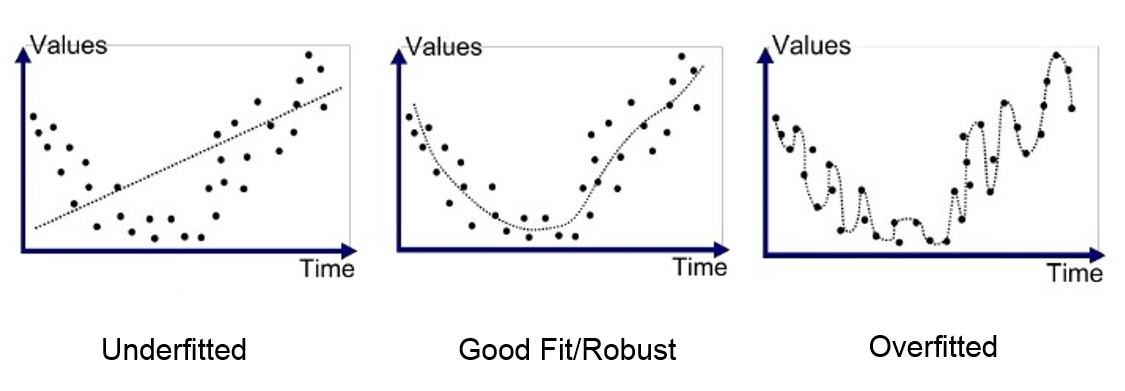
\includegraphics[width=\textwidth]{imgs/overfitting.png}
	\caption{Simplified illustration of the overfitting problem \cite{cit:overfitting}.}
	\label{label:overfitting}
\end{figure}
During the training the training accuracy of the model went above 90 \% before reaching one third of the training dataset. Indicating that the model was learning very quickly. This fact resulted in employing a different strategy to the training of the model.\\


First step was to reduce the size of the model. This was an experimental approach that included removing and reducing the convolutional layers and reducing the number of units in the dense layers. Also reducing the learning rate of the model to make convergence slower. \\

The number of epochs was increased to 200 and every epoch takes only 1/200 of the dataset, while performing validation at the end of each epoch.  Also a model checkpointing was introduced at the end of each epoch to save the model with the highest validation accuracy if required in further training or for further usage as the classification model.\\

The model was incrementally reduced and trained again to obtain the smallest model that performed the best in terms of accuracy. This process takes time to perform all the training and validation but it helps to develop basic intuition and knowledge about the dataset. The models performance was judged every step by the highest validation accuracy it can achieve. The reduction was over when the model was not able to achieve over 90\% of validation accuracy.\\

The architecture of the reduced model that performed the best can be seen in Figure \ref{label:reduced_model}. The achieved validation accuracy was 93.73\% when trained on the CNR dataset and 91.40\% when trained on PKLot dataset.\\

With this new base model obtained a fine grained tuning is employed. Such as experimenting with batch size, input size, changing the parameters of the max pooling layers, different optimizers and learning rate.


\begin{figure}[ht!]
	\centering
	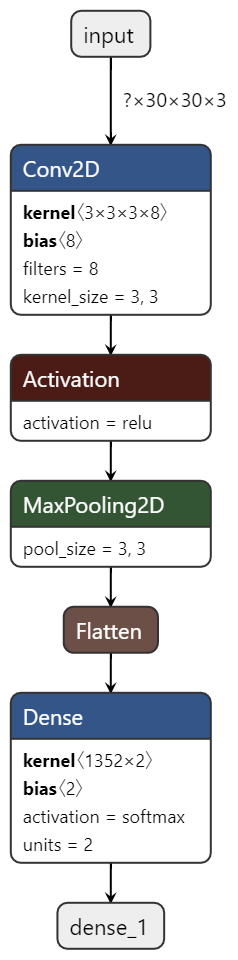
\includegraphics[scale=0.3]{imgs/reduced-model.png}
	\caption{Architecture of the reduced model. }
	\label{label:reduced_model}
\end{figure}


Adjusting the learning rate, batch size and trying different optimizers didn't improve the validation accuracy. Decreasing the input size to (width = 30, height = 30) did improve the validation accuracy. So did increasing the strides from (2, 2) to (3, 3) in the MaxPooling layer.\\

Last improvement in validation accuracy was increasing the number of strides in the first convolution layer to (5, 5). Further increase in filters, units of the dense layer or adding another convolution layer did not yield any improvement. The resulting validation accuracy was 95.88\% when trained on CNR dataset and 93.76\% when trained on PKLot dataset. The final architecture of the model can be seen in Figure \ref{label:reduced_mode_finall}. This model trained on the CNR dataset was used as classifier in the implementation.\\






\begin{figure}[ht!]
	\centering
	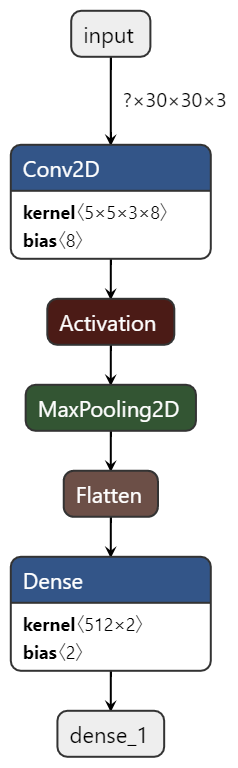
\includegraphics[scale=0.3]{imgs/reduced-model-final.png}
	\caption{Architecture of the final used classification model.}
	\label{label:reduced_mode_finall}
\end{figure}

Also five of the predefined Keras models mentioned above were picked and trained the same way to see how they perform. The results may be seen in Table \ref{label:keras_models_results}. MobileNet and ResNet50 were able to learn with around 90\% of validation accuracy. MobileNetV2 performed well while training but the validation accuracy was about 50\%.  VGG16 and VGG19 weren't able to learn at all.

\begin{table}[ht!]
\centering
\caption{Training results of five predefined Keras models. \texttt{A} is accuracy on training dataset and \texttt{VA} is validation accuracy on the other dataset.}
\begin{tabular}{|l|l|l|l|l|}
\hline
                     & \multicolumn{2}{l|}{\textbf{Trained on PKLot}} & \multicolumn{2}{l|}{\textbf{Trained on CNR}} \\ \hline
\textbf{}            & \textbf{A}            & \textbf{VA}            & \textbf{A}           & \textbf{VA}           \\ \hline
\textbf{MobileNet}   & 0.9855                & 0.8839                 & 0.9472               & 0.8649                \\ \hline
\textbf{MobileNetV2} & 0.9697                & 0.5034                 & 0.8877               & 0.4983                \\ \hline
\textbf{VGG16}       & 0.4951                & 0.5010                 & 0.4962               & 0.4962                \\ \hline
\textbf{VGG19}       & 0.4905                & 0.4945                 & 0.5013               & 0.5009                \\ \hline
\textbf{ResNet50}    & 0.9839                & 0.8913                 & 0.9661               & 0.8965                \\ \hline
\end{tabular}
\label{label:keras_models_results}
\end{table}










\section{Web application}
The web application, also reffered to as frontend, is written in JavaScript using Vue.js framework. Vue.js is an open-source progressive framework for building user interfaces created by Evan You in 2014 and is now managed by its community. \\

The actual design of the web application closely reflects the designed wireframes from the previous chapter achieved by using the Vuetify library. Vuetify provides Vue.js semantic implementations of material design components (such as buttons, forms, sliders, etc.) as well as support for the responsivity on different screen sizes via grid system based on Flexbox CSS library.\\

Frontend consumes the backend REST API using promise based library called \texttt{axios} and utilizes library called \texttt{Chart.js} to display the raw data coming from the API into charts.\\

The webpage is implemented as single-page application, meaning the default loading of a new pages mechanic in the browser is bypassed and the framework manipulates with DOM (Document Object Model) in order to display new content instead of loading a new page. It also manipulates the address bar of the browser accordingly. In this implementation the Vue router component is used to handle the route mapping and route parameters.

\subsection{Dashboard}
Dashboard is the homepage of the application. Upon opening it asynchronously queries the backend API for the information about all the parking lots registered into the system along with the most recent history entry in order to display the number of occupied and vacant spots.\\

Once the layouts for the parking lots are rendered, another asynchronous call is dispatched to backend in order to display the image of the parking lot from the camera specified as the video source. If the camera doesn't respond, an image with error notice is returned.\\

The button for adding new parking lot is always on top, after clicking it a form for adding new parking lot is opened. Whole layout of the parking lot on the dashboard is also clickable and opens the detail of the parking lot when clicked.\\

The screenshot of the dashboard on large screen can be seen in Figure \ref{label:ss_dashboard_large}. Screenshot of the menu and the dashboard on a small mobile screen may be seen in Figure \ref{label:ss_dashboard_small}.
\begin{figure}[ht!]
	\centering
	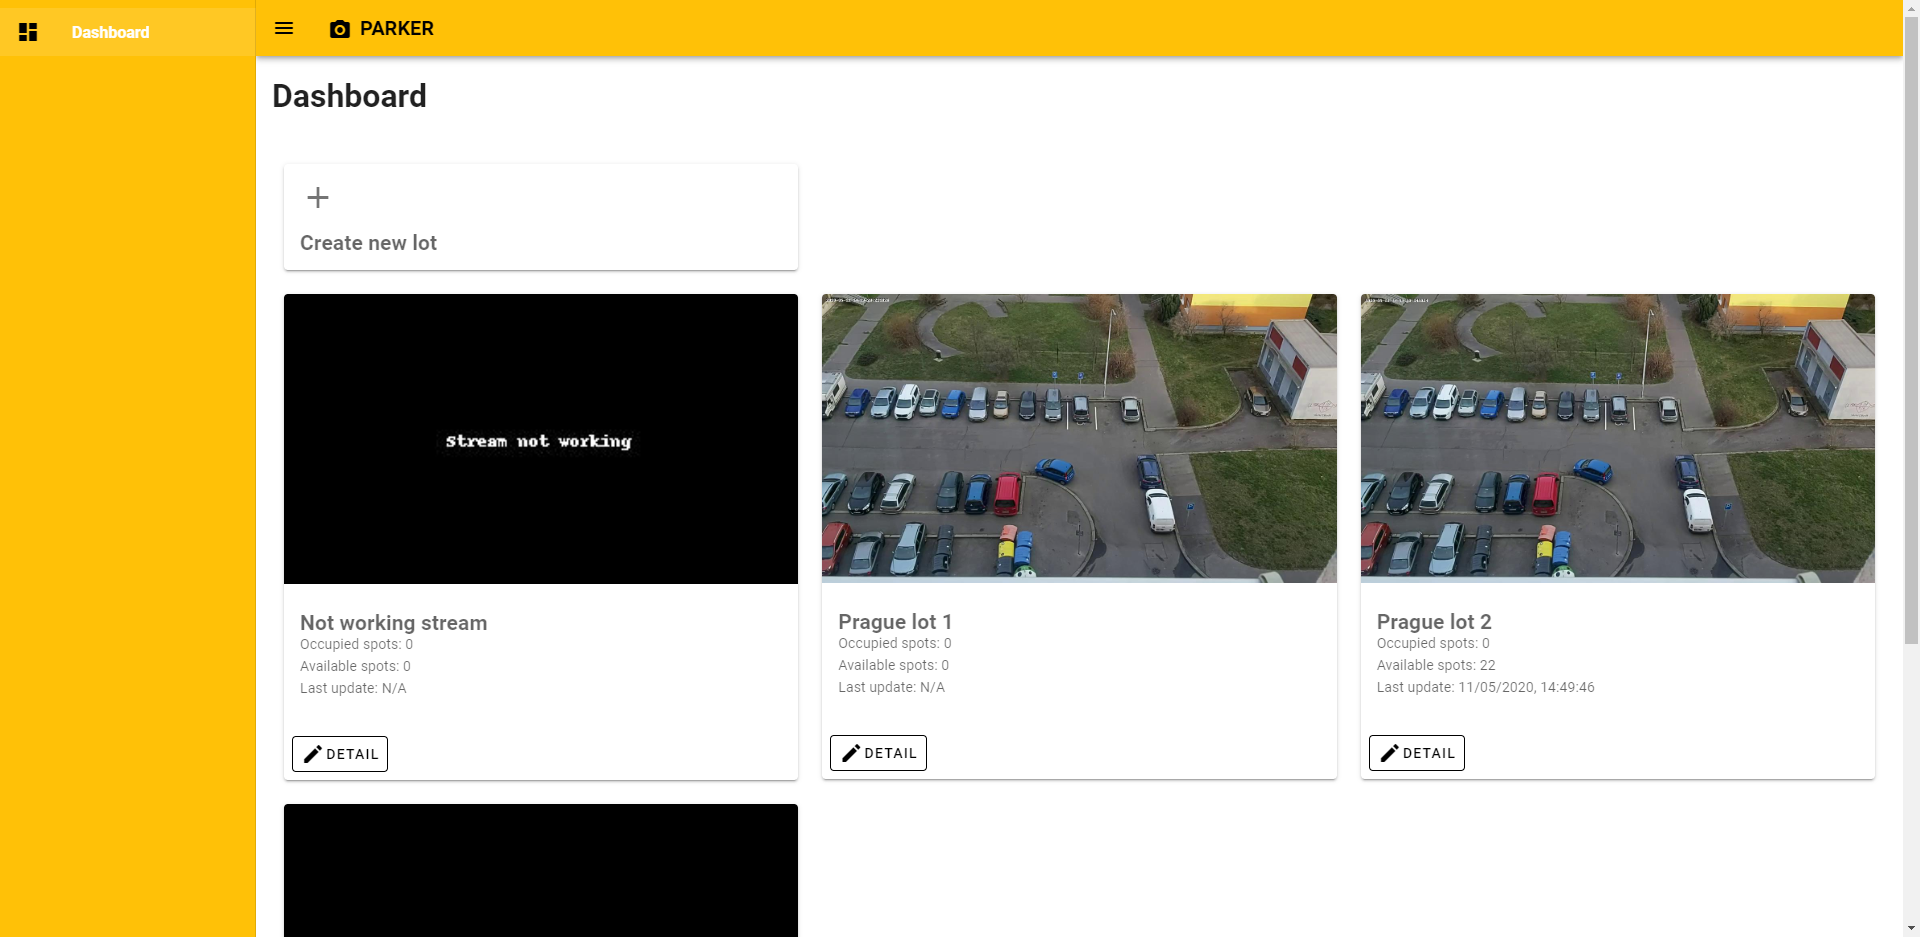
\includegraphics[scale=0.4, angle=90]{imgs/ss-dashboard.png}
	\caption{Screenshot of the dashboard page on desktop (large) screen with expanded menu.}
	\label{label:ss_dashboard_large}
\end{figure}
\begin{figure}[ht!]
	\centering
	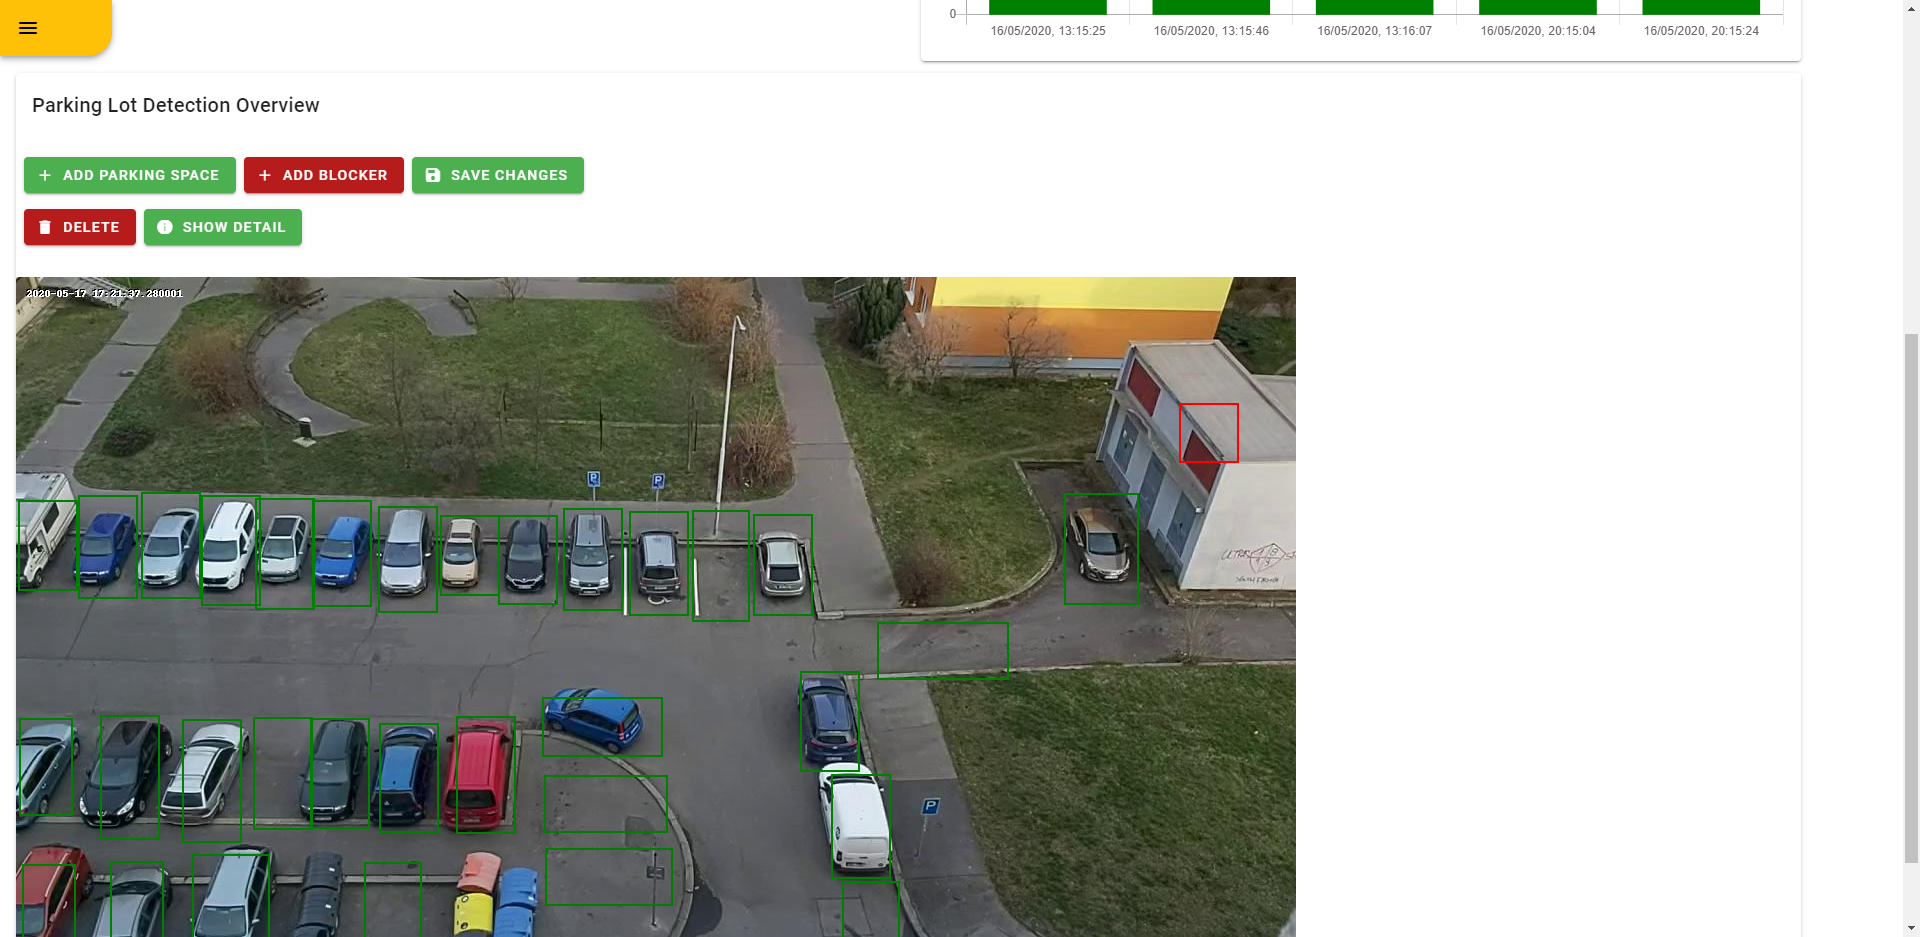
\includegraphics[scale=0.4, angle=90]{imgs/ss-detail.png}
	\caption{Screenshot of the parking lot layout on large screen.}
	\label{label:ss_dashboard_large}
\end{figure}
\begin{figure}[ht]
	\centering
	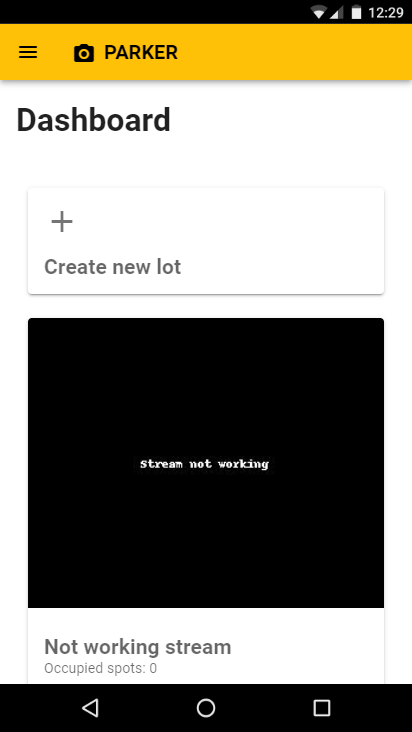
\includegraphics[width=0.45\textwidth]{imgs/ss-mobile-dashboard.png}
	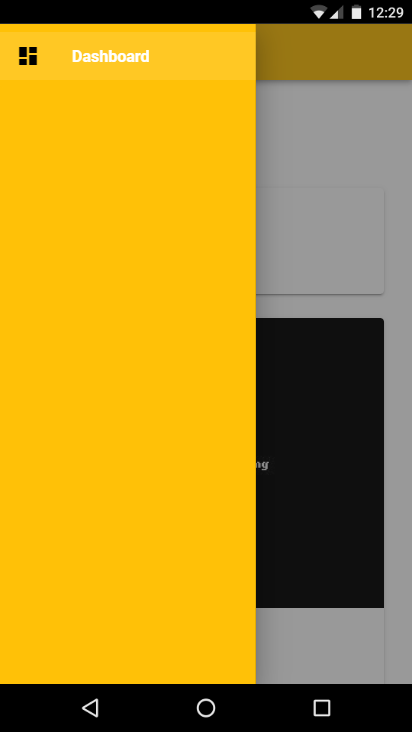
\includegraphics[width=0.45\textwidth]{imgs/ss-mobile-menu.png}
	\caption{Screenshots of the dashboard (left) and application menu (right) on a small screen.}
	\label{label:ss_dashboard_small}
\end{figure}
\subsection{Parking lot and spot detail}
The parking lot detail is located at \textbf{/lot/\texttt{id}} resource where the \texttt{id} is passed from the dashboard. The backend is then queried for the parking lots detail, history, settings, camera image and its parking spots.\\

The image and actual number of occupied and vacant spots is taken the same way as on the dashboard. The whole history of the parking lot is transformed to an object structure displayable in a chart.\\


The drag and drop tool for adjusting the parking lot layout is created using \texttt{Fabric.js} canvas library. The parking lot image is used as background for the canvas and the parking spot coordinates retrieved from backend are used to draw selectable, draggable and resizable rectangles. The buttons \texttt{Add parking space} and \texttt{Add blocker} create a new canvas rectangle when clicked. Only one selected rectangle can be deleted. All the changes need to be saved using a button \texttt{Save changes} and the new layout is propagated into the database using the backend API. Red rectangle is a blocker, yellow rectangle is a detected space that has not been acknowledged yet and green rectangle is an acknowledged parking spot.\\

After selecting an acknowledged parking spot and clicking \texttt{Show detail} button an asynchronous request is sent to the backend to retrieve history for the particular parking spot. The history is showed in a chart similar to the parking lot history in a dialog popup window.\\

The settings is implemented as a right side menu accessible by clicking the gear icon in the top right corner of the screen. The adjustable settings by the user are detection TTL for parking spots, the URI of the video source and if the detection for this parking lot should run or not. All the changes need to be saved by clicking on the \texttt{Save} button.


\begin{figure}[ht]
	\centering
		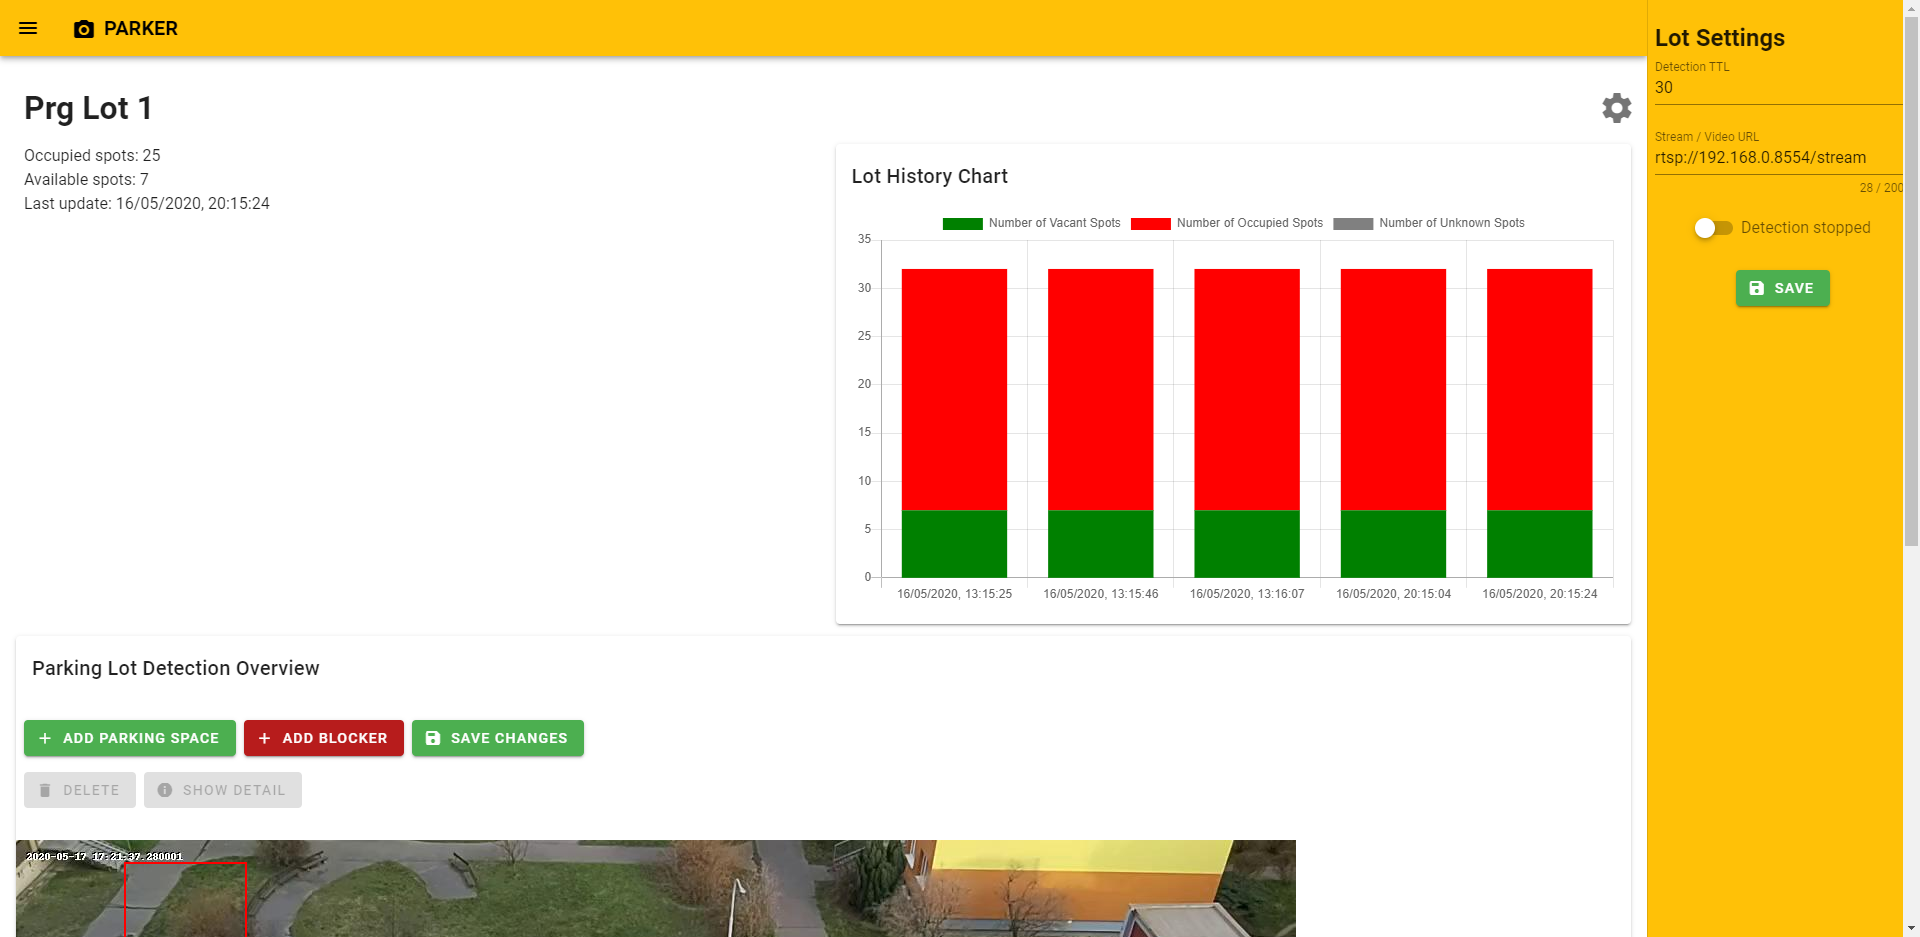
\includegraphics[scale=0.25]{imgs/ss-settings.png}
	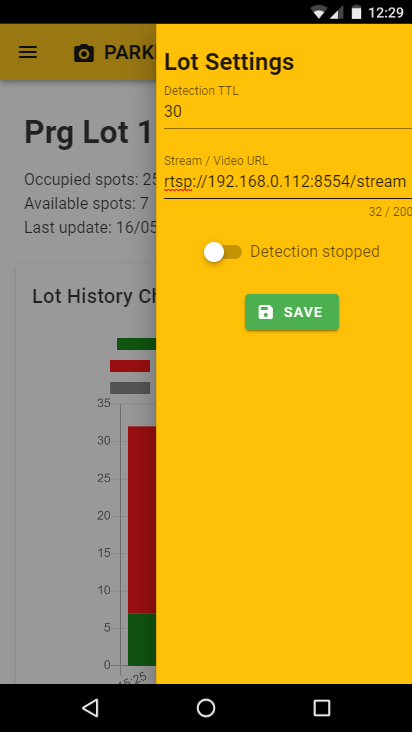
\includegraphics[scale=0.5]{imgs/ss-mobile-settings.png}
	\caption{Screenshots of the parking lot detail and settings on a large screen (top) and small screen (bottom).}
	\label{label:ss_dashboard_small}
\end{figure}
\subsection{New parking lot}
The form for adding new parking lot is located at \textbf{/addLot} resource and it is accessible from the dashboard. It only requires a name of a new parking lot and an URI of video source. Once the information is filled in and the button \texttt{Create} is clicked on a POST request is made to the backend API and the parking lot is created and visible on the dashboard. The user is notified of success or error via a popup message.\\

The screenshots of the new parking lot form on both large screens and small screens can be seen in Figure \ref{label:ss_new_both}.
\begin{figure}[ht!]
	\centering
	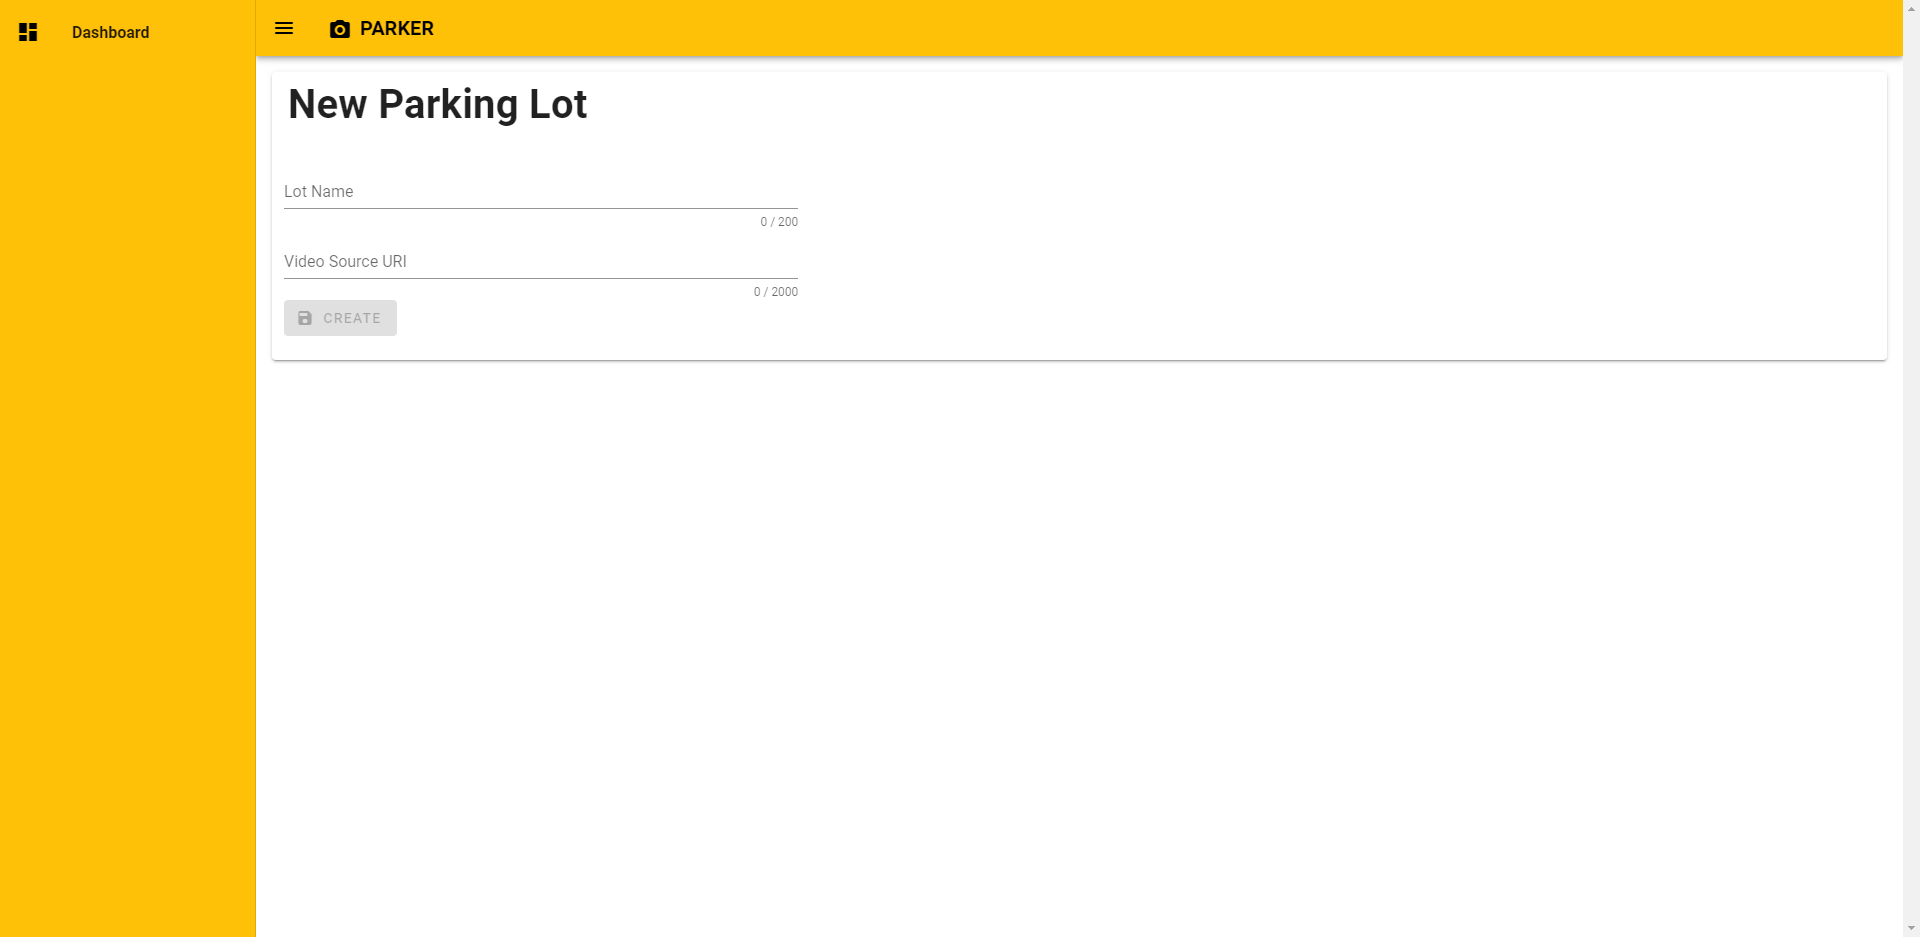
\includegraphics[scale=0.25]{imgs/ss-new.png}
	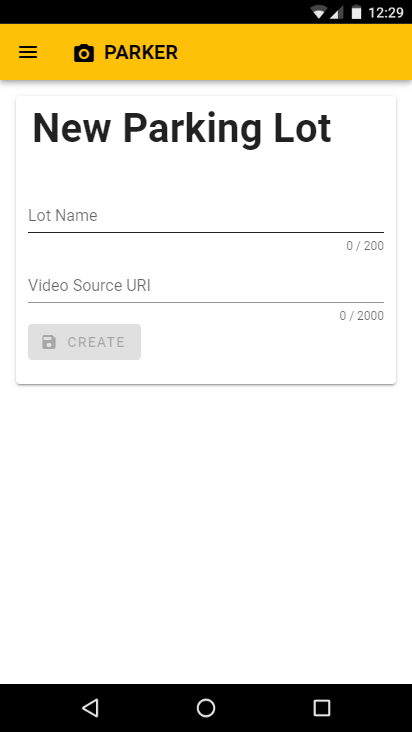
\includegraphics[scale=0.5]{imgs/ss-new-mobile.png}
	\caption{Screenshot of the form for creating a new parking lot in the application on a large screen (top) and small screen (bottom).}
	\label{label:ss_new_both}
\end{figure}

\chapter{Testing}
\section{Slicer}
The slicer implementation was tested for durability and compatibility with different video encodings. The slicer manager correctly starts and stops individual slicer processes on users demand and is able to detect if the process failed and attempts to restart it. \\


The major issue found is that the user has no feedback from the system about the type of error that happened and caused the slicer process to fail. Also using processes instead of threads has proven to be slightly more resource consuming.\\

The compatibility was tested on the custom Raspberry Pi based camera and on other publicly available IP cameras from around the world taken from the Insecam\footnote{\url{https://www.insecam.org/}} directory. The results can be seen in Table \ref{slicer_compatibility}.




\begin{table}[ht!]
\centering
\caption{Compatibility matrix of different video encodings on Windows 10 and Ubuntu Linux.}
\begin{tabular}{|l|l|l|}
\hline
\textbf{Compatibility matrix} & \textbf{Windows 10} & \textbf{Linux} \\ \hline
RTSP H.264 UDP                & No                  & Yes            \\ \hline
RTSP H.264 TCP                & Yes                 & Yes            \\ \hline
MJPEG                         & Yes                 & Yes            \\ \hline
MJPEG 4                       & Yes                 & Yes            \\ \hline
\end{tabular}
\label{slicer_compatibility}
\end{table}




\section{Object detector and spotter}
The testing of the selected Mask R-CNN object detector was already done in the analysis part of this work. Following testing was done on a footage where the cars are moving and giving right of way in the parking lot.\\

In fluid traffic the spotter performed without problems and was able to filter out the moving cars but there are few scenarios where this approach might fail.\\

The evaluation depends on the value of detection TTL setting adjustable by the user. If it is common for a particular parking lot to have cars stopping for unloading or there are queues present then it might be necessary to adjust the value of the detection TTL or mask problematic areas by blockers. Also high value of the detection TTL might lead to worse performance of the automatic detection of the parking spots.\\

In scenarios where the detection might fail the user has the option to skip the detection and delimit the parking spaces manually.




\section{Classifier}
The videos used for testing the classifier were the same as the videos for analyzing the object detectors in analysis chapter. There was also additional top view video shot at 9 PM to test the classifiers performance in poor lighting conditions.

\subsection{Top view}
The classifier performed really well on the top view examples. First top view cases may be seen in Figure \ref{label:test_top_day}, where every spot was classified correctly.\\

Second example can be seen in Figure \ref{label:test_top_night}. Most of the spots were classified correctly, except for those two spots designated for disabled people. This behavior could be expected since the datasets used for training do not contain such features.\\

Third example can be seen in Figure \ref{label:test_top2}. All the spots containing the cars were correctly classified but some free spots (marked by red rectangle) were classified incorrectly. 

\begin{figure}[ht!]
	\centering
	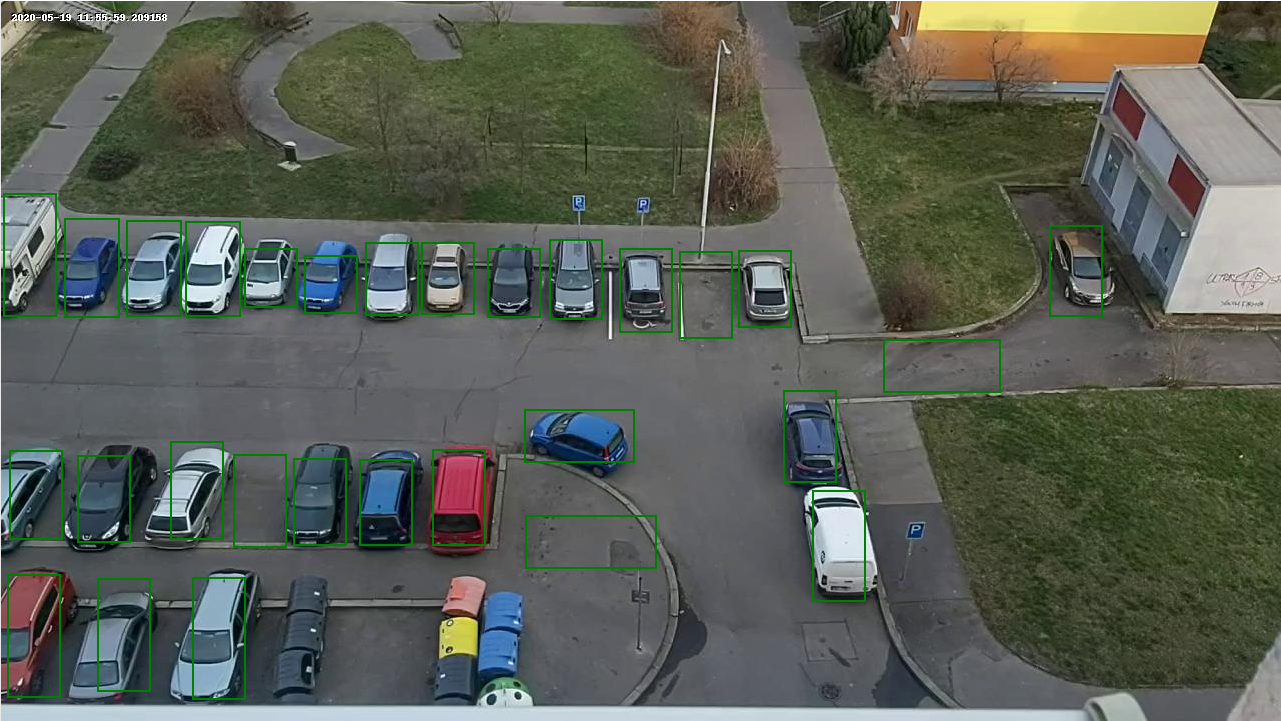
\includegraphics[width=\linewidth]{imgs/test-topview.png}
	\caption{Top view testing case during day in 1280 x 720 resolution. The achieved accuracy was 100\% on this example.}
	\label{label:test_top_day}
\end{figure}

\begin{figure}[ht!]
	\centering
	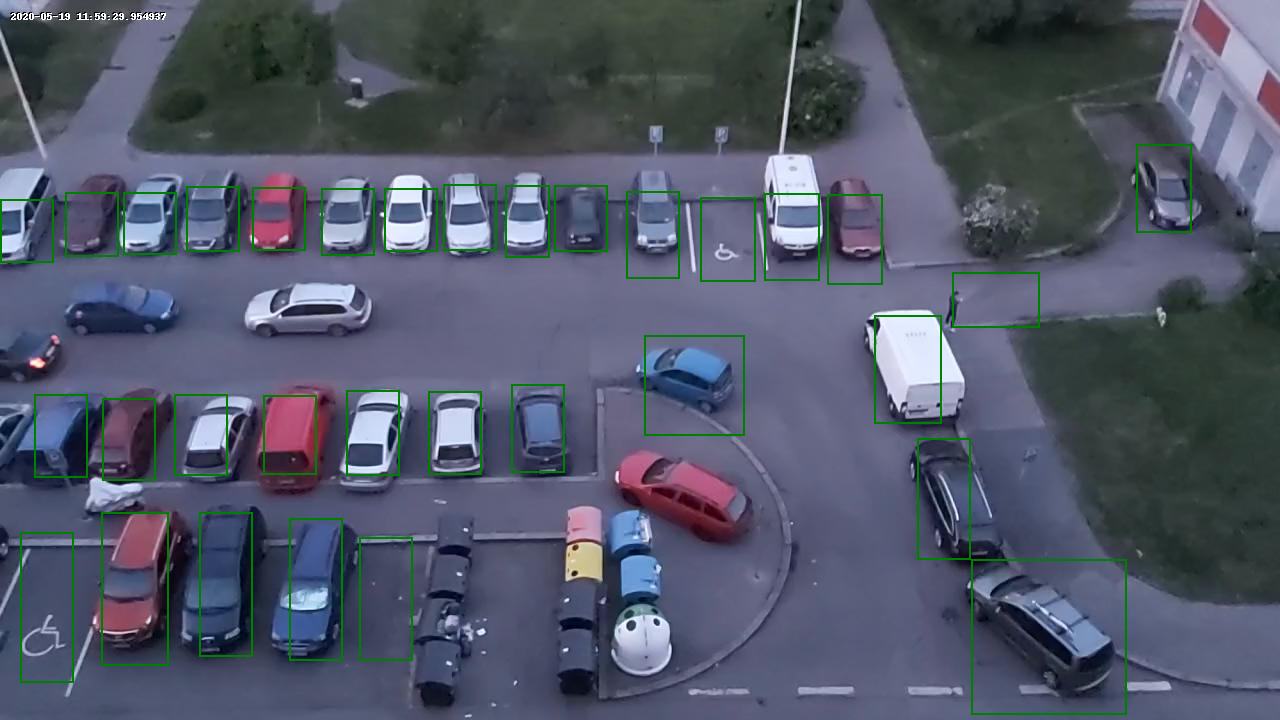
\includegraphics[width=\linewidth]{imgs/test-topview-evening.png}
	\caption{Top view testing case in 1280 x 720 resolution shot at 9 PM. Every spot was classified correctly except the two spots designated for disabled people with road markings.}
	\label{label:test_top_night}
\end{figure}
\begin{figure}[ht!]
	\centering
	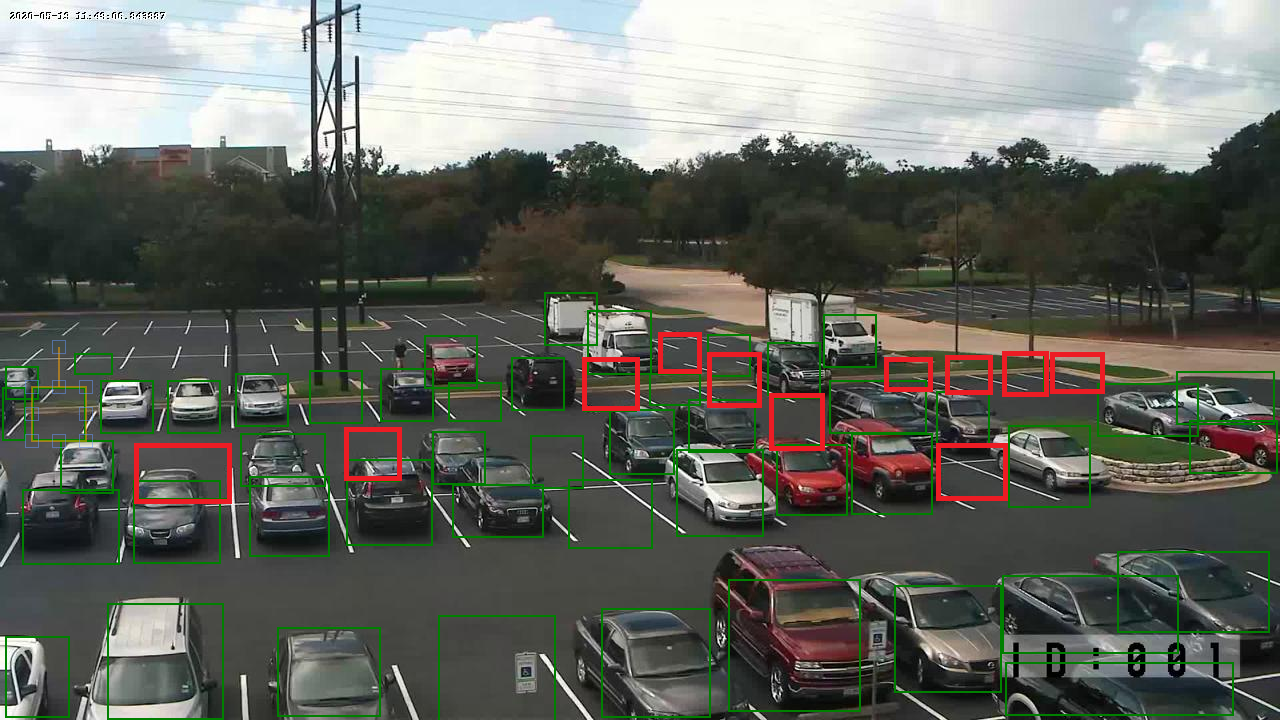
\includegraphics[width=\linewidth]{imgs/test-topview-2.png}
	\caption{Top view testing case during day in 1280 x 720 resolution. The incorrect classifications are marked with red rectangle.}
	\label{label:test_top2}
\end{figure}


\subsection{Side view}
Since the classifier accepts image in size (width = 30, height = 30) this test was performed to see if the resizing of a much larger parking spot will affect the accuracy. The result can be seen in Figure \ref{label:test_side}. The only incorrectly classified spot is marked with the red rectangle.
\begin{figure}[ht!]
	\centering
	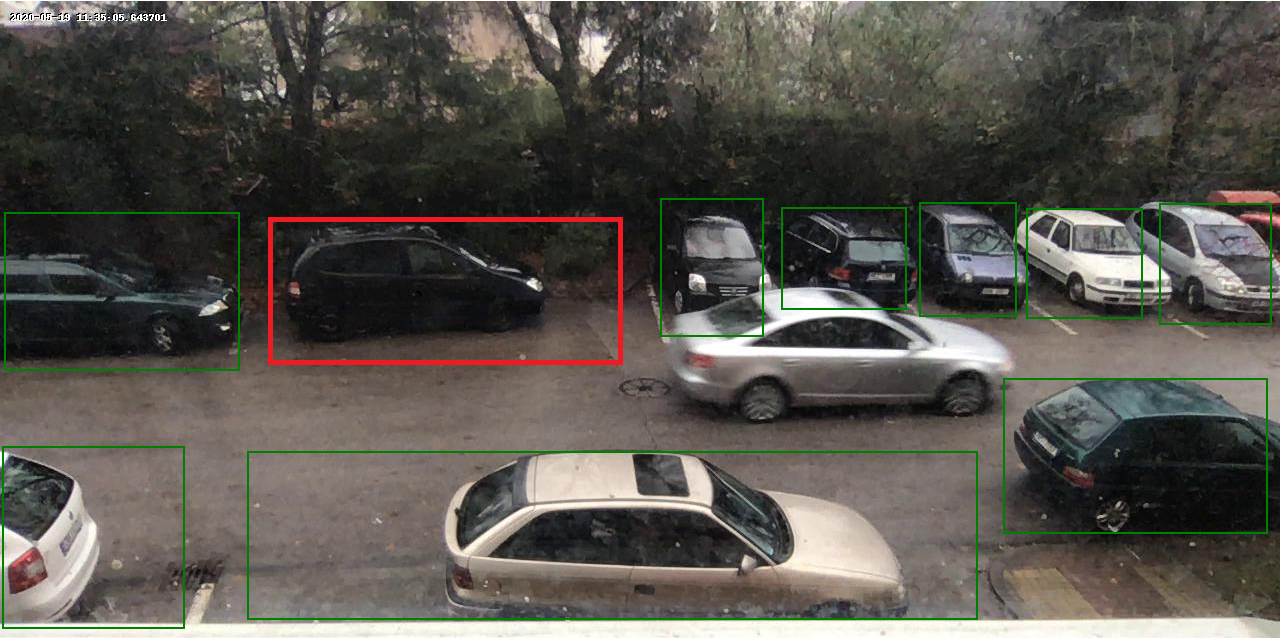
\includegraphics[width=\linewidth]{imgs/test-sideview.png}
	\caption{Side view testing case during day in a rainy weather in 1280 x 720 resolution.  The black car, marked by red rectangle, was classified incorrectly.}
	\label{label:test_side}
\end{figure}


\section{Web application}
\subsection{User Testing}
A user testing with 2 users was conducted. The first participant in user testing is Pavlína Zajícová, 23 years old student of economics. The second participant is Michal Junek, 24 years old student of software engineering.\\

The testing was performed remotely, because of the COVID-19 pandemy, on the following scenario.

\begin{enumerate}
    \item Open the main menu and make sure you are on the Dashboard.
    \item Go to the detail of \enquote{Prg Lot 1} and tell how many occupied and free parking lots are currently there. Also check if that status changed over time.
    \item Create a new parking lot with any name and with following camera URL: \textit{omitted}.
    \item Go to the newly created parking lot detail and add at least 3 parking spots and 1 new blocker. Blocker can be somewhere where it is illegal to park.
    \item Start the detection on the current parking lot. There is about 30 seconds interval to update. Change the detection TTL to 15 seconds meanwhile.
    \item Check the detail of one of the parking spots you added. Describe its status.
    \item Delete one of the parking spots.
    \item Stop the detection.
\end{enumerate}


\subsubsection{Results}
Following issues were pointed out by the users or observed from their behavior.

\begin{itemize}
    \item The newly created parking lot was not at the top of the dashboard. The user also expected to be redirected right to the detail of the new parking lot after creation.
    \item Users tried to delimit the parking lot by clicking at the top left corner of the parking spot and dragging the mouse to the bottom right corner to form a rectangle. The addition of a new parking spot to the layout wasn't noticed.
    \item Users expected the settings and parking lot layout to be saved automatically when a change was made.
    \item The settings icon was not noticed right away. The detection switch wasn't expected to be located in the settings.
    \item User missed the option to see the detail of a single parking spot.
    \item Some buttons do not provide feedback to the user after being clicked on.
\end{itemize}



\subsection{Browsers}
The web application was tested in following major browsers: Chrome (version 81.0.4044.138), Firefox (version 77.0b6), Microsoft Edge (version 44.18362.449.0), Internet Explorer 11 and Safari 13.1.\\

The websites responsivity worked as intended on Chrome, Firefox and Safari on large screens and on small screens, except for parking lot layout editor that didn't behave responsively. In Microsoft Edge and Internet Explorer there was an issue with the column dropping and the elements ended up too narrow to fit any content, making the application very hard to navigate and read.\\

The functionality testing in the browsers yielded similar results. In Chrome, Safari and Firefox on large screens the website worked properly and there was no issue. On mobile devices the parking lot layout was hard to use without the precision of a cursor. In Edge and Internet Explorer the issue was that the parking layout editor was rendered incorrectly and the rectangles delimiting the parking spots were filled with black color, rendering the component unusable.\\

\subsection{Chrome Lighthouse Audit}
This test was conducted using Chrome integrated Lighthouse tool developed by Google. Lighthouse is an automated testing tool that has audits for performance, accessibility, progressive web apps, SEO and more.\\

The tool identifies common issues with web page and displays passed and failed tests. It also provides helpful list of issues that should be checked manually.

\subsubsection{Performance}
The received grade is 0/100. The received grade was so low, because Lighthouse reported that the website took 88 seconds to load. That statement is not true as the web page loads in approximately 2 seconds. Issues found were following.
\begin{itemize}
    \item No text compression.
    \item Not using next-gen image formats such as WebP or JPEG 2000.
\end{itemize}

\subsubsection{Accessibility}
The received grade is 76/100. This test looks for sufficient contrast between colors, HTML language attributes, headings, document title, Javascript turned off in browser, etc. The only issue reported by Lighthouse was that the buttons do not have an accessible name, namely the button that opens the side menu.

\subsubsection{Best Practices}
The received grade is 83/100. This test suite checks for usage of deprecated libraries, correct aspect ratio of images, application caching, etc. The only issue found was not using passive listeners to improve scroll performance.


\chapter{Future improvements}
All the tests performed in this work definitely yielded some minor and major shortcomings that will be addressed in future. \\

One of the major issues is that the object detector is insufficient in recognizing vehicles on a wide angle footage and doesn't classify correctly enough. However, the detected occupied parking spots are input data for training the object detector. So the current object detector may be swapped in the future for a model trained using this gathered data.  \\

The classification using CNN showed a great potential but is not very precise on a crowded parking lot. Delimiting the parking spots with rectangles is not optimal when the parking spots are not perpendicular to the camera. Using polygons or rotated bounding boxes might improve the classification potential. Also enriching the datasets with more features found on parking lots might yield an improvement.\\

The frontend part had issues with browser compatibility, mainly with Microsoft products. Testing with users brought a lot of directions and topics in which the frontend will be improved to be more user friendly and intuitive. \\

So far this solution is not designed to run outside of secure network. It is planned to add authentication and security measures to allow the application to be deployed and accessible from the internet.\\






\setsecnumdepth{part}

\chapter{Conclusion}
The goal of this masters thesis was to design and implement a system that can process the video stream of a parking lot camera, extract locations of parking spots using the parked vehicles and determine the occupancy status of the parking lot.\\

The system is composed of several services and a processing pipeline that periodically takes an image from the stream, locates the vehicles using object detector and performs time based sampling in order to filter out moving vehicles and eventually acknowledge the parking spots. Acknowledged parking spots are periodically evaluated for occupancy status by a custom classifier.\\

A web application for displaying the gathered data in a human friendly manner was developed and allows the user to make changes to the parking lot layout and other settings.\\

The whole application is not working perfectly on every parking lot, there are some issues that will need to be addressed in the future. Nevertheless, the chosen approach showed a good promise and the architecture was designed with extendability and improvability in mind.





\bibliographystyle{iso690}
\bibliography{mybibliographyfile}

\setsecnumdepth{all}
\appendix
\chapter{Installation guide}

The main configuration file is located at \texttt{common/settings.py}.
\section{Preconditions}
\begin{itemize}
    \item Basic knowledge of Docker, Python with pip, Apache Kafka and networking.
    \item Recommended operating system is Linux. Windows might encounter some compability issues.
    \item Kafka/ PostgreSQL (optional)
    \item Python 3.6+ installed with pip (package installer for Python)
    \item Docker (developed on version 2.2.0.5) with \textit{docker-compose} capability
\end{itemize}


\section{Preparing the infrastructure}
\section{Contents of the configuration file}
\begin{description}
    \item [DB_NAME] The name of the database in PostgreSQL for this project.
    \item [DB_HOST] The IP address of the database.
    \item [DB_USER] The username for access to the database.
    \item [DB_PASS] The password for specified username.
    \item [KAFKA_SERVERS] List of IP addresses of Apache Kafka instances.
    \item [SLICER_CHECK_INTERVAL] Interval in seconds how often the running of slicer processes is checked.
    \item [CLASSIFY_PERIOD_SECONDS] Specifies how often are parking spots evaluated by classifier.
\end{description}


\section{Clone the repository}
Clone repository using the git command or download the repository via the GitHub website and open the directory of the project in command line.

\begin{minted}[breaklines]{bash}
git clone https://github.com/opendatalabcz/parking-spot-detection.git
\end{minted}


\section{PostgreSQL}
If you already have a running instance of PostgreSQL that you want to use then just make sure you fill the main configuration file accordingly and skip this step.\\

If you want to use the dockerized PostgreSQL open file \texttt{docker-compose.yml} and change username and password to your liking in \texttt{services/db/POSTGRES_USER and POSTGRES_PASSWORD} and adjust main configuration file accordingly or skip this step to leave default settings.\\

\section{Apache Kafka}
If you already have an Apache Kafka instance running, make sure you properly configure the maximum size of the message in Kafka configuration. The configuration can be taken from \texttt{docker-compose.yml} and skip this step.\\
TODO: needs zoopeeker notice
If you want to use dockerized Kafka instance it is setup to work right out of the box. If you wish to make changes to the configuration, it can be done in the \textit{docker-compose.yml} file.

\section{Running the services}
\section{Running the containers}
Make sure you have opened the root folder of the project in command line and run following command. Arguments in square brackets are optional. Argument \texttt{-d} will run the containers in the background.

\begin{minted}[breaklines]{bash}
docker-compose up db zookeeper kafka [pgadmin] [-d]
\end{minted}

Make sure you create database for this project in PostgreSQL and update \texttt{DB_NAME} in \texttt{common/settings.py} accordingly. The optional \textit{pgadmin} will run pgAdmin4 web based interface for managing the PostgreSQL instance. It can be used to easily create the new database.\\

Run the following command to get the ids of the running containers.
\begin{minted}{bash}
 docker ps
\end{minted}

Use the ids in the output of previous command to get the IP adresses of the containers using following command. And fill out the main configuration file accordingly.
\begin{minted}[breaklines]{bash}
docker inspect -f '{{range .NetworkSettings.Networks}}{{.IPAddress}}{{end}}' id
\end{minted}

\section{Backend}
Run the following commands for the first time setup.
\begin{minted}[breaklines]{bash}
pip install -r requirements.txt
cd backend
python manage.py migrate
\end{minted}

After the first time setup run the following commands. The output of the first command is going to contain the IP address of the backend server. This IP address needs to be assigned into variable \texttt{BACKEND_URL} in file  \texttt{frontend/api/api.js}.

\begin{minted}[breaklines]{bash}
python manage.py runserver [&]
python manage.py time_spotter [&]
python manage.py slicer [&]
\end{minted}

\section{Running the detector and classifier}
The detector and classifier can be run by following commands.
\begin{minted}[breaklines]{bash}
python detector/receive.py [&]
python park_classifier/receive.py [&]
\end{minted}

\section{Running the frontend}
The frontend can be run using following commands. The last command will output the IP address of the website.
\begin{minted}[breaklines]{bash}
cd frontend
npm ci
npm run serve
\end{minted}



\chapter{Acronyms}
% \printglossaries
\begin{description}
	\item[GUI] Graphical user interface
	\item[XML] Extensible markup language
	\item[YOLO] You Only Look Once
\end{description}


\chapter{Contents of enclosed CD}

%change appropriately

\begin{figure}
	\dirtree{%
		.1 readme.txt\DTcomment{the file with CD contents description}.
		.1 exe\DTcomment{the directory with executables}.
		.1 src\DTcomment{the directory of source codes}.
		.2 wbdcm\DTcomment{implementation sources}.
		.2 thesis\DTcomment{the directory of \LaTeX{} source codes of the thesis}.
		.1 text\DTcomment{the thesis text directory}.
		.2 thesis.pdf\DTcomment{the thesis text in PDF format}.
		.2 thesis.ps\DTcomment{the thesis text in PS format}.
	}
\end{figure}

\end{document}
